%%%%%%%%%%%%%%%%%%%%%%%%%%%%%%% beamer %%%%%%%%%%%%%%%%%%%%%%%%%%%%%%%%%%%%%%%%%%%%%%%%%
% To run - pdflatex filename.tex
%      acroread filename.pdf
%%%%%%%%%%%%%%%%%%%%%%%%%%%%%%%%%%%%%%%%%%%%%%%%%%%%%%%%%%%%%%%%%%%%%%%%%%%%%%%%%%%%%%%%

\documentclass[compress,oilve]{beamer}
\mode<presentation>

\usetheme[]{CambridgeUS}
% other themes: AnnArbor, Antibes, Bergen, Berkeley, Berlin, Boadilla, boxes, CambridgeUS, Copenhagen, Darmstadt, default, Dresden, Frankfurt, Goettingen,
% Hannover, Ilmenau, JuanLesPins, Luebeck, Madrid, Maloe, Marburg, Montpellier, PaloAlto, Pittsburg, Rochester, Singapore, Szeged, classic

\usecolortheme{beaver}
% color themes: albatross, beaver, beetle, crane, default, dolphin,  fly, lily, orchid, rose, seagull, seahorse, sidebartab, whale, wolverine

\usefonttheme{professionalfonts}
% font themes: default, professionalfonts, serif, structurebold, structureitalicserif, structuresmallcapsserif


\hypersetup{pdfpagemode=FullScreen} % makes your presentation go automatically to full screen

% define your own colors:
\definecolor{Red}{rgb}{1,0,0}
\definecolor{Blue}{rgb}{0,0,1}
\definecolor{Green}{rgb}{0,1,0}
\definecolor{magenta}{rgb}{1,0,.6}
\definecolor{lightblue}{rgb}{0,.5,1}
\definecolor{lightpurple}{rgb}{0.8, 0.6, 0.9}
\definecolor{gold}{rgb}{.6,.5,0}
\definecolor{orange}{rgb}{1,0.4,0}
\definecolor{hotpink}{rgb}{1,0,0.5}
\definecolor{newcolor2}{rgb}{.5,.3,.5}
\definecolor{newcolor}{rgb}{0,.3,1}
\definecolor{newcolor3}{rgb}{1,0,.35}
\definecolor{darkgreen1}{rgb}{0, .35, 0}
\definecolor{darkgreen}{rgb}{0, .6, 0}
\definecolor{darkred}{rgb}{.75,0,0}
\definecolor{skyblue}{HTML}{75bbfd}

\definecolor{olive}{cmyk}{0.64,0,0.95,0.4}
\definecolor{purpleish}{cmyk}{0.75,0.75,0,0}

% can also choose different themes for the "inside" and "outside"

% \usepackage{beamerinnertheme_______}
% inner themes include circles, default, inmargin, rectangles, rounded

% \usepackage{beamerouterthemesmoothbars}
% outer themes include default, infolines, miniframes, shadow, sidebar, smoothbars, smoothtree, split, tree


\useoutertheme[subsection=true, height=40pt]{smoothbars}

% to have the same footer on all slides
%\setbeamertemplate{footline}[text line]{STUFF HERE!}
\setbeamertemplate{footline}[text line]{} % makes the footer EMPTY
% include packages
%

%show the page numbers in footnote
%\addtobeamertemplate{navigation symbols}{}{%
%	\usebeamerfont{footline}%
%	\usebeamercolor[fg]{footline}%
%	\hspace{1em}%
%	\insertframenumber/\inserttotalframenumber
%}

\setbeamercolor{footline}{fg=purpleish}
\setbeamerfont{footline}{series=\bfseries}

%add color to curent subsection
\setbeamertemplate{section in head/foot}{\hfill\tikz\node[rectangle, fill=darkred, rounded corners=1pt,inner sep=1pt,] {\textcolor{white}{\insertsectionhead}};}
\setbeamertemplate{section in head/foot shaded}{\textcolor{darkred}{\hfill\insertsectionhead}}

% Remove bullet of subsections
\setbeamertemplate{headline}
{%
	\begin{beamercolorbox}{section in head/foot}
		\insertsectionnavigationhorizontal{\textwidth}{}{}
	\end{beamercolorbox}%
}


% modify headlline, specially headline size
\setbeamertemplate{headline}{%
	\leavevmode%
	\hbox{%
		\begin{beamercolorbox}[wd=\paperwidth,ht=3.5ex,dp=1.125ex]{palette quaternary}%
			\insertsectionnavigationhorizontal{\paperwidth}{}{\hskip0pt plus1filll}
		\end{beamercolorbox}%
	}
}

\setbeamertemplate{footline}{%
	\leavevmode%
	\hbox{\begin{beamercolorbox}[wd=.5\paperwidth,ht=2.5ex,dp=1.125ex,leftskip=.3cm plus1fill,rightskip=.3cm]{author in head/foot}%
			\usebeamerfont{author in head/foot}\insertshortauthor ~ \insertshortinstitute
		\end{beamercolorbox}%
		\begin{beamercolorbox}[wd=.5\paperwidth,ht=2.5ex,dp=1.125ex,leftskip=.3cm,rightskip=.3cm plus1fil]{title in head/foot}%
			\usebeamerfont{title in head/foot}\insertshorttitle\hfill\insertframenumber\,/\,\inserttotalframenumber
	\end{beamercolorbox}}%
	\vskip0pt%
}


%\setbeamertemplate{navigation symbols}{}

\title{CNN Architecture}
\author{ML Instruction Team, Fall 2022}
\institute[]{CE Department \newline  Sharif University of Technology \newline \newline \newline
            Ali Sharifi-Zarchi \newline
            Behrooz Azarkhalili \newline
            Arian Amani \newline
            Hamidreza Yaghoubi}
\date[\today]{}
%\titlegraphic{\includegraphics[scale=.35]{example-image}}



%Write \usepackage{etex} just after the \documentclass line (it should be the first loaded package).
\usepackage{etex}
\usepackage{subcaption}
\usepackage{caption}
\usepackage{multicol}
\usepackage{amsmath}
\usepackage{epsfig}
\usepackage{graphicx}
\usepackage[all,knot]{xy}
\xyoption{arc}
\usepackage{url}
\usepackage{multimedia}
\usepackage{hyperref}
\hypersetup{colorlinks,linkcolor=blue,citecolor=red,urlcolor=darkred}
\usepackage{multirow}
\usepackage[font={scriptsize}]{caption}
\usepackage{pgf}
\usepackage{fontspec}
\usepackage{svg}

% \usepackage{biblatex}
% \addbibresource{Refrences.bib}
% \AtBeginBibliography{\small}


%\setsansfont[Scale=MatchLowercase, BoldFont = * Bold, ItalicFont = * Italic]{Caladea}

%\usepackage{enumitem,xcolor}
%\newcommand{\labelitemi}{$\blacksquare$}
%\newcommand{\labelitemii}{$\diamond$}
%\newcommand{\labelitemiii}{$\square$}
%\newcommand{\labelitemiv}{$\ast$}
%\setbeamercolor*{item}{fg=red}

% abbreviation
% \newrobustcmd{\B}{\bfseries}

\usefonttheme{professionalfonts} 
\setbeamertemplate{itemize item}{\color{skyblue}$\blacksquare$}
\setbeamertemplate{itemize subitem}{\color{hotpink}$\blacktriangleright$}
\setbeamertemplate{itemize subsubitem}{\color{orange}$\bullet$}


\usepackage{anyfontsize}
\usepackage{t1enc}
\usepackage{tikz}
\usetikzlibrary{calc,trees,positioning,arrows,chains,shapes.geometric,decorations.pathreplacing,decorations.pathmorphing,shapes,matrix,shapes.symbols}



\newtheorem{proposition}[theorem]{Proposition}
\newtheorem{remark}[theorem]{Remark}
\newtheorem{assumption}[theorem]{Assumption}

\usepackage{xcolor}
\newcommand{\tc}[2]{
	\textcolor{#1}{#2}
}

%\usepackage{fontspec, unicode-math}
%\setmainfont[Scale=0.9]{Nimbus Roman No9 L}
%\setmonofont[Scale=0.9]{Monaco}
\setsansfont[Scale=1]{Times New Roman}

\newcommand{\vect}[1]{\boldsymbol{#1}}

\definecolor{strings}{rgb}{.624,.251,.259}
\definecolor{keywords}{rgb}{.224,.451,.686}
\definecolor{comment}{rgb}{.322,.451,.322}


%\usepackage{smartdiagram}
%\usesmartdiagramlibrary{additions}
%%%%%%%%%%%%%%%%%%%%%%%%%%%%%%%%%%%%%%%%%%%%%%%%%%%%%%%%%%%%%%%%%%%%%%%%%%%%%%%%%%%%%%%%%%%%
%%%%%%%%%%%%%%%%%%%%%%%%%%%%%% Title Page Info %%%%%%%%%%%%%%%%%%%%%%%%%%%%%%%%%%%%%%%%%%%
%%%%%%%%%%%%%%%%%%%%%%%%%%%%%%%%%%%%%%%%%%%%%%%%%%%%%%%%%%%%%%%%%%%%%%%%%%%%%%%%%%%%%%%%%%


%%%%%%%%%%%%%%%%%%%%%%%%%%%%%%%%%%%%%%%%%%%%%%%%%%%%%%%%%%%%%%%%%%%%%%%%%%%%%%%%%%%%%%%%%%
%%%%%%%%%%%%%%%%%%%%%%%%%%%%%% Begin Your Document %%%%%%%%%%%%%%%%%%%%%%%%%%%%%%%%%%%%%%%
%%%%%%%%%%%%%%%%%%%%%%%%%%%%%%%%%%%%%%%%%%%%%%%%%%%%%%%%%%%%%%%%%%%%%%%%%%%%%%%%%%%%%%%%%%
\begin{document}
	
%%%%%%%%%%%%%%%%%%%%%%%%%%%%%%%%%%%%%%%%%%%%%%%%%%%%%%%%%%%%%%%%%%%%%%%%%%%%%%%%%%%%%%%%%%
	\fontsize{9}{9}
\begin{frame}[noframenumbering, plain]
	\titlepage
\end{frame}

%%%%%%%%%%%%%%%%%%%%%%%%%%%%%%%%%%%%%%%%%%%%%%%%%%%%%%%%%%%%%%%%%%%%%%%%%%%%%%%%%%%%%%%%%%
\section{Introduction}
%%%%%%%%%%%%%%%%%%%%%%%%%%%%%%%%%%%%%%%%%%%%%%%%%%%%%%%%%%%%%%%%%%%%%%%%%%%%%%%%%%%%%%%%%%

\frame{\frametitle{Brief History of Computer Vision}

\Large{What is Computer Vision?}

\begin{figure}
\centering
\begin{minipage}{.5\textwidth}
  \centering
    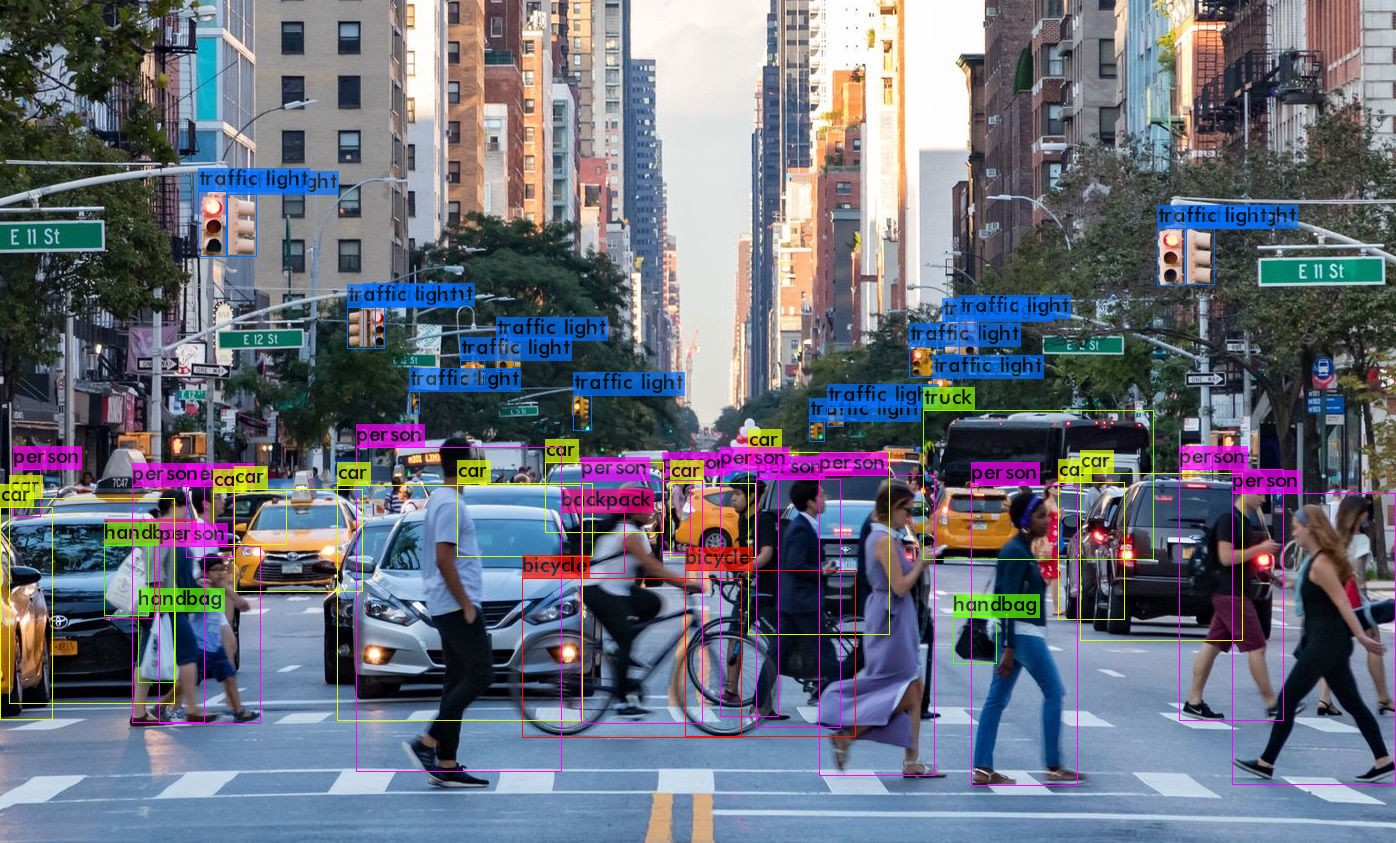
\includegraphics[width=0.65\columnwidth]{images/intro1.jpeg} \caption{\href{https://alexeyab84.medium.com/yolov4-the-most-accurate-real-time-neural-network-on-ms-coco-dataset-73adfd3602fe}{Source}}
\end{minipage}%
\begin{minipage}{.5\textwidth}
  \centering
    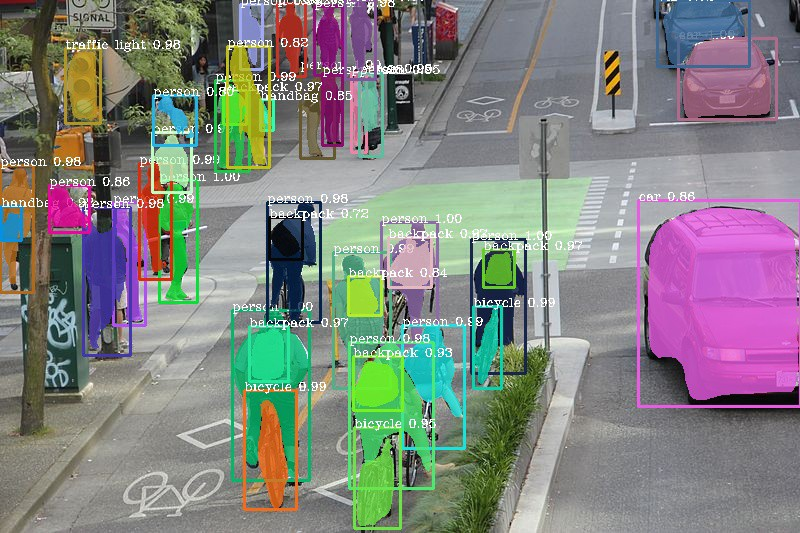
\includegraphics[width=0.65\columnwidth]{images/intro3.jpeg}
    \caption{\href{https://towardsdatascience.com/image-segmentation-with-six-lines-0f-code-acb870a462e8}{Source}}
\end{minipage}
\newline
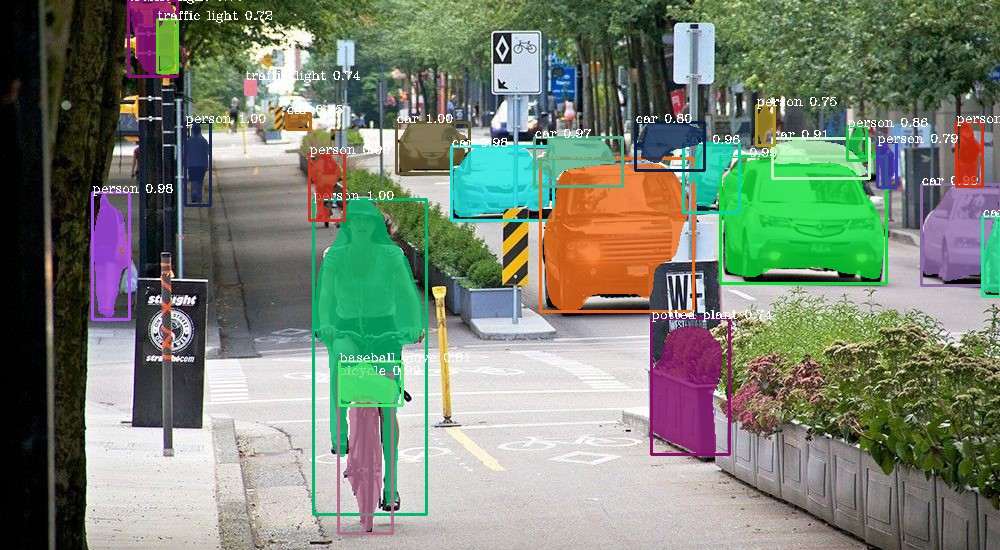
\includegraphics[width=0.35\columnwidth]{images/intro2.jpeg}
\caption{\href{https://miro.medium.com/max/1000/1*81e42V29ALfP6eU1FPhMdg.jpeg}{Source}}
\end{figure}
}

%%%%%%%%%%%%%%%%%%%%%%%%%%%%%%%%%%%%%%%%%%%%%%%%%%%%%%%%%%%%%%%%%%%%%%%%%%%%%%%%%%%%%%%%%%

\frame{\frametitle{Brief History of Computer Vision}

\Large{Before Deep Learning:} \large{\tc{keywords}{Hand-Crafted Features}}

\begin{figure}
    \centering
    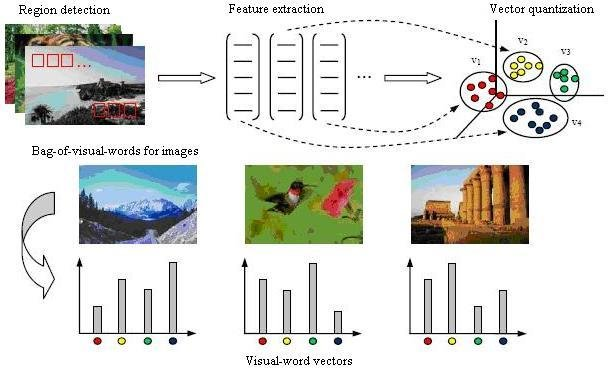
\includegraphics[width=0.8\columnwidth]{images/intro4.jpg} \caption{\cite{featureextrac2013}}
\end{figure}
}

%%%%%%%%%%%%%%%%%%%%%%%%%%%%%%%%%%%%%%%%%%%%%%%%%%%%%%%%%%%%%%%%%%%%%%%%%%%%%%%%%%%%%%%%%%

\frame{\frametitle{Brief History of Computer Vision}

\Large{Before Deep Learning:} \large{\tc{keywords}{Hand-Crafted Features}}

\begin{figure}
    \centering
    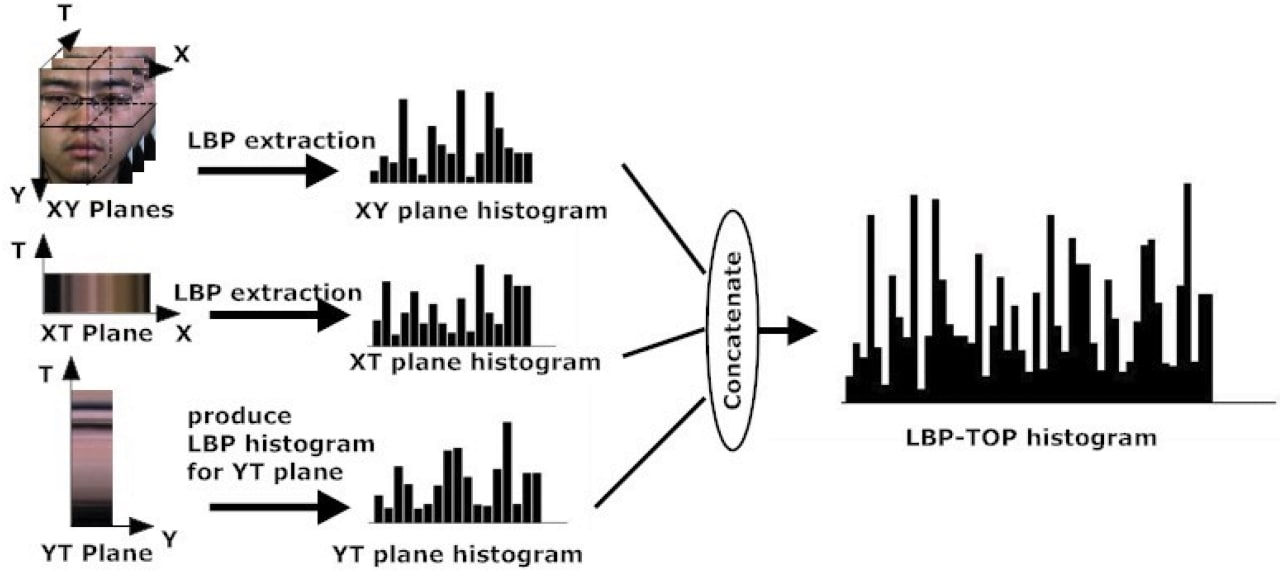
\includegraphics[width=0.9\columnwidth]{images/intro5.jpg}
    \caption{\cite{wang_see_phan_oh_2015}}
\end{figure}
}

%%%%%%%%%%%%%%%%%%%%%%%%%%%%%%%%%%%%%%%%%%%%%%%%%%%%%%%%%%%%%%%%%%%%%%%%%%%%%%%%%%%%%%%%%%

\frame{\frametitle{Brief History of Computer Vision}

\Large{Effect of Deep Learning:} \large{\tc{keywords}{Comparison between Deep Learning and Traditional Models}}

\begin{figure}
    \centering
    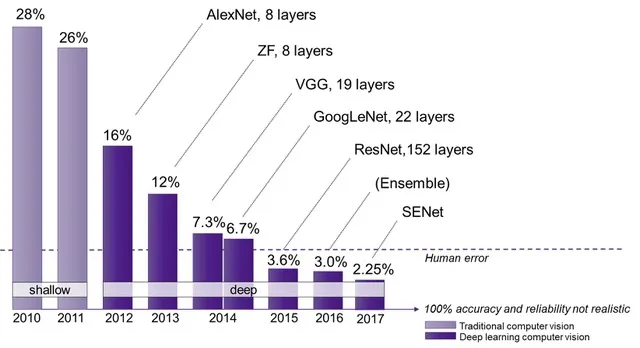
\includegraphics[width=0.85\columnwidth]{images/intro6.png}
    \caption{ImageNet Competetion Results Over Time, \href{https://semiengineering.com/new-vision-technologies-for-real-world-applications/}{Source}}
\end{figure}
}

%%%%%%%%%%%%%%%%%%%%%%%%%%%%%%%%%%%%%%%%%%%%%%%%%%%%%%%%%%%%%%%%%%%%%%%%%%%%%%%%%%%%%%%%%

\frame{\frametitle{CNNs}

\Large{What we've been using:}
\newline\newline
\large{- Fully Connected Layers}
\newline
\begin{figure}
    \centering
    \includesvg[width=1\columnwidth]{images/nn.svg}
\end{figure}
}


%%%%%%%%%%%%%%%%%%%%%%%%%%%%%%%%%%%%%%%%%%%%%%%%%%%%%%%%%%%%%%%%%%%%%%%%%%%%%%%%%%%%%%%%%%%%%%%
\section{Kernels}
%%%%%%%%%%%%%%%%%%%%%%%%%%%%%%%%%%%%%%%%%%%%%%%%%%%%%%%%%%%%%%%%%%%%%%%%%%%%%%%%%%%%%%%%%%%%%%%

\frame{\frametitle{CNNs}

\Large{What we're going to learn:}
\newline\newline
\large{- Convolutional Layer}
\newline
\begin{figure}
    \centering
    \includesvg[width=0.6\columnwidth]{images/CNN1.svg}
\end{figure}

}

%%%%%%%%%%%%%%%%%%%%%%%%%%%%%%%%%%%%%%%%%%%%%%%%%%%%%%%%%%%%%%%%%%%%%%%%%%%%%%%%%%%%%%%%%%%%%%%

\frame{\frametitle{CNNs vs. FCNs}
\centering\Large{First of all...}
}
%%%%%%%%%%%%%%%%%%%%%%%%%%%%%%%%%%%%%%%%%%%%%%%%%%%%%%%%%%%%%%%%%%%%%%%%%%%%%%%%%%%%%%%%%%%%%%%

\frame{\frametitle{CNNs vs. FCNs}
\centering\large{Why use ConvNets instead of Fully Connected Networks with images?}
}

%%%%%%%%%%%%%%%%%%%%%%%%%%%%%%%%%%%%%%%%%%%%%%%%%%%%%%%%%%%%%%%%%%%%%%%%%%%%%%%%%%%%%%%%%%%%%%%

\frame{\frametitle{CNNs vs. FCNs}
\centering\Large{Let's do an experiment.}
}

%%%%%%%%%%%%%%%%%%%%%%%%%%%%%%%%%%%%%%%%%%%%%%%%%%%%%%%%%%%%%%%%%%%%%%%%%%%%%%%%%%%%%%%%%%%%%%%

\frame{\frametitle{CNNs vs. FCNs}
\centering\Large{We're going to use the CIFAR10 dataset}
\begin{figure}
    \centering
    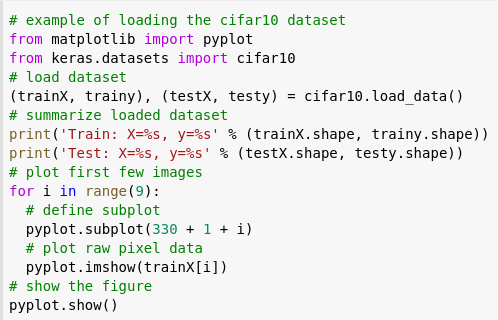
\includegraphics[width=0.8\columnwidth]{images/intro8.png}
\end{figure}
}

%%%%%%%%%%%%%%%%%%%%%%%%%%%%%%%%%%%%%%%%%%%%%%%%%%%%%%%%%%%%%%%%%%%%%%%%%%%%%%%%%%%%%%%%%%%%%%%

\frame{\frametitle{CNNs vs. FCNs}
\centering\Large{We're going to use the CIFAR10 dataset}
\begin{figure}
    \centering
    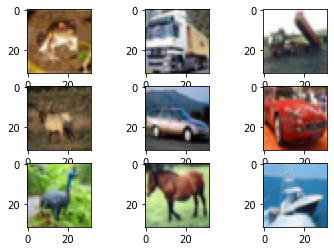
\includegraphics[width=0.7\columnwidth]{images/intro7.png}
\end{figure}
}


%%%%%%%%%%%%%%%%%%%%%%%%%%%%%%%%%%%%%%%%%%%%%%%%%%%%%%%%%%%%%%%%%%%%%%%%%%%%%%%%%%%%%%%%%%%%%%%

\frame{\frametitle{CNNs vs. FCNs}
\centering\large{First, we train on a Fully Connected Network}
\begin{figure}
    \centering
    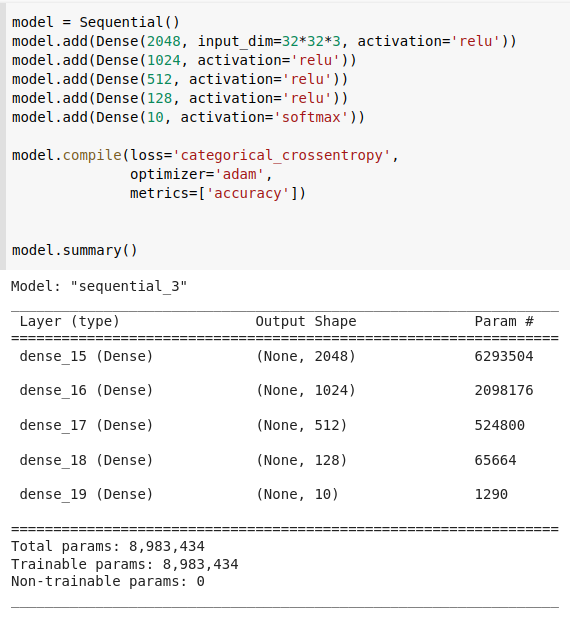
\includegraphics[width=0.45\columnwidth]{images/intro9.png}
    \caption{FCN with around 9M parameters}
\end{figure}
}

%%%%%%%%%%%%%%%%%%%%%%%%%%%%%%%%%%%%%%%%%%%%%%%%%%%%%%%%%%%%%%%%%%%%%%%%%%%%%%%%%%%%%%%%%%%%%%%

\frame{\frametitle{CNNs vs. FCNs}
\centering\Large{First, we train on a Fully Connected Network}
\begin{figure}
    \centering
    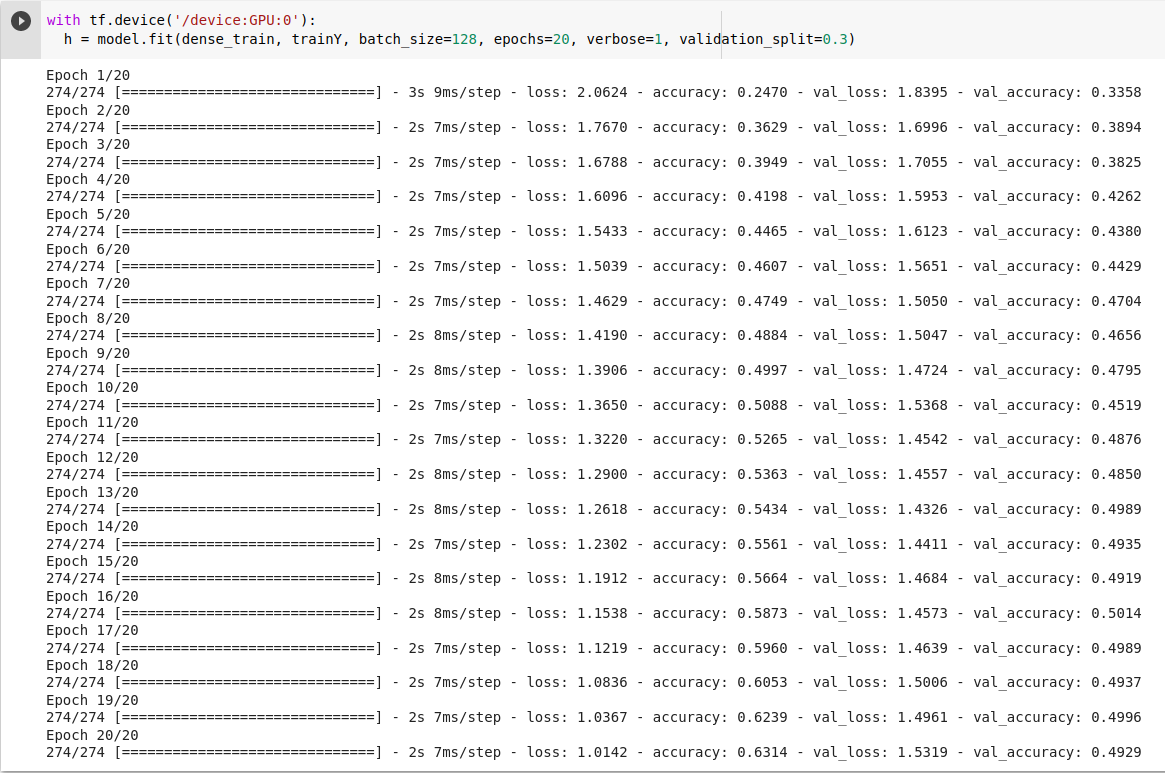
\includegraphics[width=0.7\columnwidth]{images/intro10.png}
    \caption{Training for 20 epochs}
\end{figure}
}

%%%%%%%%%%%%%%%%%%%%%%%%%%%%%%%%%%%%%%%%%%%%%%%%%%%%%%%%%%%%%%%%%%%%%%%%%%%%%%%%%%%%%%%%%%%%%%%

\frame{\frametitle{CNNs vs. FCNs}
\centering\Large{First, we train on a Fully Connected Network}
\begin{figure}
    \centering
    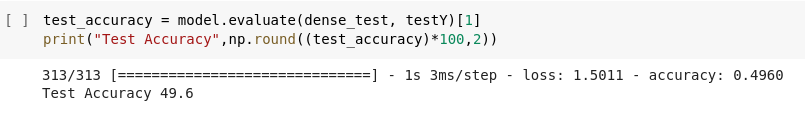
\includegraphics[width=0.9\columnwidth]{images/intro11.png}
    \caption{Test results after the training is done; Test Accuracy = 49.6\%}
\end{figure}
}

%%%%%%%%%%%%%%%%%%%%%%%%%%%%%%%%%%%%%%%%%%%%%%%%%%%%%%%%%%%%%%%%%%%%%%%%%%%%%%%%%%%%%%%%%%%%%%%

\frame{\frametitle{CNNs vs. FCNs}
\centering\large{Now, let's train on a Convolutional Neural Network}
\begin{figure}
    \centering
    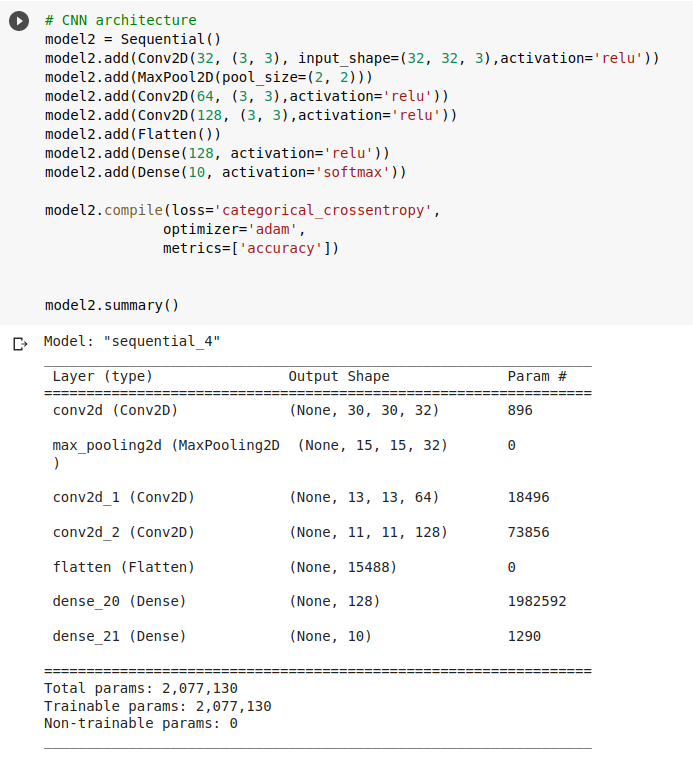
\includegraphics[width=0.45\columnwidth]{images/intro12.png}
    \caption{CNN with around 2M parameters (A lot less compared to our 9M parameter FCN)}
\end{figure}
}

%%%%%%%%%%%%%%%%%%%%%%%%%%%%%%%%%%%%%%%%%%%%%%%%%%%%%%%%%%%%%%%%%%%%%%%%%%%%%%%%%%%%%%%%%%%%%%%

\frame{\frametitle{CNNs vs. FCNs}
\centering\Large{Now, let's train on a Convolutional Neural Network}
\begin{figure}
    \centering
    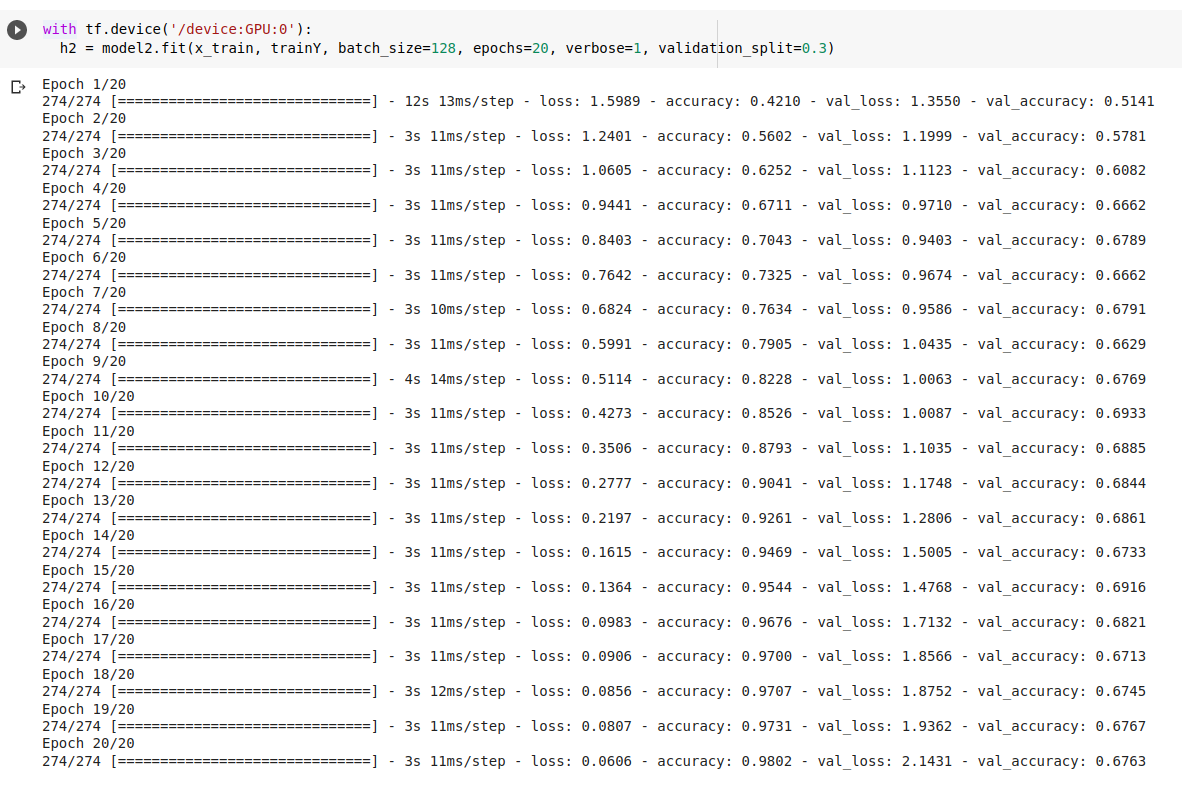
\includegraphics[width=0.7\columnwidth]{images/intro13.png}
    \caption{Training for 20 epochs}
\end{figure}
}

%%%%%%%%%%%%%%%%%%%%%%%%%%%%%%%%%%%%%%%%%%%%%%%%%%%%%%%%%%%%%%%%%%%%%%%%%%%%%%%%%%%%%%%%%%%%%%%

\frame{\frametitle{CNNs vs. FCNs}
\centering\Large{Now, let's train on a Convolutional Neural Network}
\begin{figure}
    \centering
    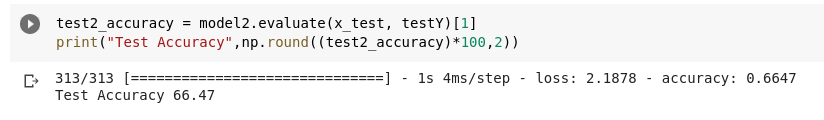
\includegraphics[width=0.9\columnwidth]{images/intro14.png}
    \caption{Test results after the training is done; Test Accuracy = 66.5\%}
\end{figure}
}

%%%%%%%%%%%%%%%%%%%%%%%%%%%%%%%%%%%%%%%%%%%%%%%%%%%%%%%%%%%%%%%%%%%%%%%%%%%%%%%%%%%%%%%%%%%%%%%

\frame{\frametitle{CNNs vs. FCNs}
\begin{itemize}
    \item \large As you can see, CNNs have a great effect on both results and computation efficiency while working with visual imagery.
\end{itemize}
\newline
\begin{center}
\begin{tabular}{||c | c | c||} 
 \hline
 Model Architecture & \# Params & Test Accuracy \\ [0.5ex] 
 \hline\hline
 \normalsize \textbf{CNN} & \normalsize \textbf{2M} & \normalsize \textbf{66.5\%} \\ 
 \hline
 \normalsize FCN & \normalsize 9M & \normalsize 49.6\% \\ [1ex] 
 \hline
\end{tabular}
\end{center}
}

%%%%%%%%%%%%%%%%%%%%%%%%%%%%%%%%%%%%%%%%%%%%%%%%%%%%%%%%%%%%%%%%%%%%%%%%%%%%%%%%%%%%%%%%%%%%%%%

\frame{\frametitle{CNNs vs. FCNs}
\centering\Large{Now that we understand the importance of Deep Learning and 
Convolutional Neural Networks, let's learn the details.}
}

%%%%%%%%%%%%%%%%%%%%%%%%%%%%%%%%%%%%%%%%%%%%%%%%%%%%%%%%%%%%%%%%%%%%%%%%%%%%%%%%%%%%%%%%%%%%%%%

\frame{\frametitle{CNNs}

\large{Convolutional Layer}
\newline

\begin{itemize}
	\item Filters always extend the full depth of the input.\newline
	(\#Input channels == \#Filter Channels)
\end{itemize}	

\begin{figure}
    \centering
    \includesvg[width=0.6\columnwidth]{images/CNN2.svg}
\end{figure}

}


%%%%%%%%%%%%%%%%%%%%%%%%%%%%%%%%%%%%%%%%%%%%%%%%%%%%%%%%%%%%%%%%%%%%%%%%%%%%%%%%%%%%%%%%%%%%%%%

\frame{\frametitle{What is Convolution and how does it work?}
\normalsize
\begin{itemize}
    \item \color{red}We apply the same filter on different regions of the input
\end{itemize}
\begin{figure}
    \centering
    \includesvg[width=0.6\columnwidth]{images/kernel2.svg}
\end{figure}

}

%%%%%%%%%%%%%%%%%%%%%%%%%%%%%%%%%%%%%%%%%%%%%%%%%%%%%%%%%%%%%%%%%%%%%%%%%%%%%%%%%%%%%%%%%%%%%%%

\frame{\frametitle{What is Convolution and how does it work?}
\normalsize

\begin{itemize}
    \item We apply the same filter on different regions of the input
    \item \color{red} Convolutional filters learn to make decisions based on local spatial input, which is an important attribute when working with images.
\end{itemize}
\begin{figure}
    \centering
    \includesvg[width=0.6\columnwidth]{images/kernel3.svg}
\end{figure}

}

%%%%%%%%%%%%%%%%%%%%%%%%%%%%%%%%%%%%%%%%%%%%%%%%%%%%%%%%%%%%%%%%%%%%%%%%%%%%%%%%%%%%%%%%%%%%%%%

\frame{\frametitle{What is Convolution and how does it work?}
\normalsize

\begin{itemize}
    \item We apply the same filter on different regions of the input
    \item Convolutional filters learn to make decisions based on local spatial input, which is an important attribute when working with images.
    \item \color{red} Uses a lot fewer parameters compared to Fully Connected Layers.
\end{itemize}
\begin{figure}
    \centering
    \includesvg[width=0.6\columnwidth]{images/kernel4.svg}
\end{figure}

}

%%%%%%%%%%%%%%%%%%%%%%%%%%%%%%%%%%%%%%%%%%%%%%%%%%%%%%%%%%%%%%%%%%%%%%%%%%%%%%%%%%%%%%%%%%%%%%%

\frame{\frametitle{What is Convolution and how does it work?}
\normalsize
Consider this, the filter we are going to use:
\begin{figure}
    \centering
    \includesvg[width=0.45\columnwidth]{images/kernel5.svg}
\end{figure}
}

%%%%%%%%%%%%%%%%%%%%%%%%%%%%%%%%%%%%%%%%%%%%%%%%%%%%%%%%%%%%%%%%%%%%%%%%%%%%%%%%%%%%%%%%%%%%%%%

\foreach \i in {0,...,8}
{
    \frame{\frametitle{What is Convolution and how does it work?}
    \normalsize
    This is how we calculate the convolutional layer's output:
    \small
    \begin{equation*}
        Convolved Feature(i, j) = (I * K)(i, j) = \sum_{a=0}^{k_h - 1}\sum_{b=0}^{k_w - 1} I(i+a, j+b) K(a, b)
    \end{equation*}
        I: Input Image\newline
        K: Our Kernel\newline
        $k_h$ and $k_w$: The height and width of the Kernel

    \begin{figure}
    \centering
    \begin{minipage}{.7\textwidth}
      \centering
        \includegraphics[width=0.5\columnwidth]{images/kernel-frame-\i.png}
        \caption{Convoluting a 5x5x1 image with a 3x3x1 kernel to get a 3x3x1 convolved feature, \href{https://towardsdatascience.com/a-comprehensive-guide-to-convolutional-neural-networks-the-eli5-way-3bd2b1164a53}{Source}}
    \end{minipage}%
    \begin{minipage}{.3\textwidth}
      \centering
        \includesvg[width=0.45\columnwidth]{images/kernel6.svg}
        \caption{Convolving Kernel}
    \end{minipage}


    \end{figure}
    }
}
%%%%%%%%%%%%%%%%%%%%%%%%%%%%%%%%%%%%%%%%%%%%%%%%%%%%%%%%%%%%%%%%%%%%%%%%%%%%%%%%%%%%%%%%%%%%%%%
\section{Strides}
%%%%%%%%%%%%%%%%%%%%%%%%%%%%%%%%%%%%%%%%%%%%%%%%%%%%%%%%%%%%%%%%%%%%%%%%%%%%%%%%%%%%%%%%%%%%%%%
\frame{\frametitle{What is a Stride}

\Large{The amount of movement between applications of the filter to the input image is referred to as the stride, and it is almost always symmetrical in height and width dimensions.}
\newline
\newline
\normalsize{Closer look}
\begin{itemize}
	\item 7x7 input with 3x3 filter
\end{itemize}	

\begin{figure}
    \centering
    \includesvg[width=0.35\columnwidth]{images/Stride1.svg}
\end{figure}

}

%%%%%%%%%%%%%%%%%%%%%%%%%%%%%%%%%%%%%%%%%%%%%%%%%%%%%%%%%%%%%%%%%%%%%%%%%%%%%%%%%%%%%%%%%%%%%%%

\frame{\frametitle{What is a Stride}

\Large{The amount of movement between applications of the filter to the input image is referred to as the stride, and it is almost always symmetrical in height and width dimensions.}
\newline
\newline
\normalsize{Closer look}
\begin{itemize}
	\item 7x7 input with 3x3 filter
\end{itemize}	

\begin{figure}
    \centering
    \includesvg[width=0.35\columnwidth]{images/Stride2.svg}
\end{figure}

}

%%%%%%%%%%%%%%%%%%%%%%%%%%%%%%%%%%%%%%%%%%%%%%%%%%%%%%%%%%%%%%%%%%%%%%%%%%%%%%%%%%%%%%%%%%%%%%%

\frame{\frametitle{What is a Stride}

\Large{The amount of movement between applications of the filter to the input image is referred to as the stride, and it is almost always symmetrical in height and width dimensions.}
\newline
\newline
\normalsize{Closer look}
\begin{itemize}
	\item 7x7 input with 3x3 filter
\end{itemize}	

\begin{figure}
    \centering
    \includesvg[width=0.35\columnwidth]{images/Stride3.svg}
\end{figure}

}

%%%%%%%%%%%%%%%%%%%%%%%%%%%%%%%%%%%%%%%%%%%%%%%%%%%%%%%%%%%%%%%%%%%%%%%%%%%%%%%%%%%%%%%%%%%%%%%

\frame{\frametitle{What is a Stride}

\Large{The amount of movement between applications of the filter to the input image is referred to as the stride, and it is almost always symmetrical in height and width dimensions.}
\newline
\newline
\normalsize{Closer look}
\begin{itemize}
	\item 7x7 input with 3x3 filter
\end{itemize}	

\begin{figure}
    \centering
    \includesvg[width=0.35\columnwidth]{images/Stride4.svg}
\end{figure}

}

%%%%%%%%%%%%%%%%%%%%%%%%%%%%%%%%%%%%%%%%%%%%%%%%%%%%%%%%%%%%%%%%%%%%%%%%%%%%%%%%%%%%%%%%%%%%%%%

\frame{\frametitle{What is a Stride}

\Large{The amount of movement between applications of the filter to the input image is referred to as the stride, and it is almost always symmetrical in height and width dimensions.}
\newline
\newline
\normalsize{Closer look}
\begin{itemize}
	\item 7x7 input with 3x3 filter
	\item This was a Stride 1 filter
	\item=> Outputs 5x5
\end{itemize}	

\begin{figure}
    \centering
    \includesvg[width=0.3\columnwidth]{images/Stride5.svg}
\end{figure}

}


%%%%%%%%%%%%%%%%%%%%%%%%%%%%%%%%%%%%%%%%%%%%%%%%%%%%%%%%%%%%%%%%%%%%%%%%%%%%%%%%%%%%%%%%%%%%%%%

\frame{\frametitle{Strides}

\newline
\newline
\normalsize{\color{red}Now let's use Stride 2}
\begin{itemize}
	\item 7x7 input with 3x3 filter

\end{itemize}	

\begin{figure}
    \centering
    \includesvg[width=0.35\columnwidth]{images/Stride6.svg}
\end{figure}
}

%%%%%%%%%%%%%%%%%%%%%%%%%%%%%%%%%%%%%%%%%%%%%%%%%%%%%%%%%%%%%%%%%%%%%%%%%%%%%%%%%%%%%%%%%%%%%%%

\frame{\frametitle{Strides}

\newline
\newline
\normalsize{Now let's use Stride 2}
\begin{itemize}
	\item 7x7 input with 3x3 filter

\end{itemize}	

\begin{figure}
    \centering
    \includesvg[width=0.35\columnwidth]{images/Stride7.svg}
\end{figure}
}

%%%%%%%%%%%%%%%%%%%%%%%%%%%%%%%%%%%%%%%%%%%%%%%%%%%%%%%%%%%%%%%%%%%%%%%%%%%%%%%%%%%%%%%%%%%%%%%

\frame{\frametitle{Strides}

\newline
\newline
\normalsize{Now let's use Stride 2}
\begin{itemize}
	\item 7x7 input with 3x3 filter
	\item This was a Stride 2 filter
	\item=> Outputs 3x3
\end{itemize}	

\begin{figure}
    \centering
    \includesvg[width=0.3\columnwidth]{images/Stride8.svg}
\end{figure}
}

%%%%%%%%%%%%%%%%%%%%%%%%%%%%%%%%%%%%%%%%%%%%%%%%%%%%%%%%%%%%%%%%%%%%%%%%%%%%%%%%%%%%%%%%%%%%%%%

\frame{\frametitle{Strides}

\newline
\newline
\normalsize{\color{red}Stride 3?}
\begin{itemize}
	\item 7x7 input with 3x3 filter

\end{itemize}	

\begin{figure}
    \centering
    \includesvg[width=0.25\columnwidth]{images/Stride9.svg}
    \includesvg[width=0.25\columnwidth]{images/Stride10.svg}
    \includesvg[width=0.34\columnwidth]{images/Stride11.svg}
\end{figure}
}
%%%%%%%%%%%%%%%%%%%%%%%%%%%%%%%%%%%%%%%%%%%%%%%%%%%%%%%%%%%%%%%%%%%%%%%%%%%%%%%%%%%%%%%%%%%%%%%

\frame{\frametitle{Strides}

\newline
\newline
\normalsize{\color{red}So 7x7 input with 3x3 filter and stride 3 doens't work!}
\newline
\newline
\large{Let't do the calculations:}
\newline \newline
\large{$Output Size = (N - F) / Stride + 1$}

\begin{figure}
    \centering
    \includesvg[width=0.4\columnwidth]{images/Stride12.svg}
\end{figure}
}

%%%%%%%%%%%%%%%%%%%%%%%%%%%%%%%%%%%%%%%%%%%%%%%%%%%%%%%%%%%%%%%%%%%%%%%%%%%%%%%%%%%%%%%%%%%%%%%

\frame{\frametitle{Strides}
\newline
\newline
\large{$Output Size = (N - F) / Stride + 1$}

N = 7, F = 3 =>
\begin{itemize}
    \item Stride 1 ==> $(7 - 3) / 1 + 1 = 5$
    \item Stride 2 ==> $(7 - 3) / 2 + 1 = 3$
    \item \color{red}Stride 3 ==> $(7 - 3) / 3 + 1 = 2.33$ :))
\end{itemize}
\begin{figure}
    \centering
    \includesvg[width=0.4\columnwidth]{images/Stride12.svg}
\end{figure}
}

%%%%%%%%%%%%%%%%%%%%%%%%%%%%%%%%%%%%%%%%%%%%%%%%%%%%%%%%%%%%%%%%%%%%%%%%%%%%%%%%%%%%%%%%%%%%%%%
\frame{\frametitle{Strides}
\begin{center}
    \LARGE{Do you see any problems?}
\end{center}
}

%%%%%%%%%%%%%%%%%%%%%%%%%%%%%%%%%%%%%%%%%%%%%%%%%%%%%%%%%%%%%%%%%%%%%%%%%%%%%%%%%%%%%%%%%%%%%%%
\frame{\frametitle{Strides}
\begin{center}
    \begin{itemize}
        \item\color{red}\Large{1. Borders don't get enough attention.}
    \end{itemize}
    \begin{figure}
        \centering
        \includesvg[width=0.9\columnwidth]{images/padding1.svg}
        \caption{\cite{zhang2021dive}, Pixel utilization for convolutions of size $1 \times 1$, $2 \times 2$, and $3 \times 3$ respectively.}
        % \label{fig:my_label}
    \end{figure}
\end{center}
}

%%%%%%%%%%%%%%%%%%%%%%%%%%%%%%%%%%%%%%%%%%%%%%%%%%%%%%%%%%%%%%%%%%%%%%%%%%%%%%%%%%%%%%%%%%%%%%%
\frame{\frametitle{Strides}
\begin{center}
    \begin{itemize}
        \item\Large{1. Borders don't get enough attention.}
        \item\color{red}\Large{2. Outputs shrink!}
    \end{itemize}
    \begin{figure}
        \centering
        \includesvg[width=0.9\columnwidth]{images/Padding2.svg}
        \caption{32x32 input shrinks to 28x28 output. (information loss)}
        % \label{fig:my_label}
    \end{figure}
\end{center}
}

%%%%%%%%%%%%%%%%%%%%%%%%%%%%%%%%%%%%%%%%%%%%%%%%%%%%%%%%%%%%%%%%%%%%%%%%%%%%%%%%%%%%%%%%%%%%%%%
\frame{\frametitle{Strides}
\begin{center}
    \LARGE{What is the solution?}
\end{center}
}

%%%%%%%%%%%%%%%%%%%%%%%%%%%%%%%%%%%%%%%%%%%%%%%%%%%%%%%%%%%%%%%%%%%%%%%%%%%%%%%%%%%%%%%%%%%%%%%
\section{Padding}
%%%%%%%%%%%%%%%%%%%%%%%%%%%%%%%%%%%%%%%%%%%%%%%%%%%%%%%%%%%%%%%%%%%%%%%%%%%%%%%%%%%%%%%%%%%%%%%
\frame{\frametitle{Padding}
\begin{center}
    \LARGE{Enters Padding}
\end{center}
}

%%%%%%%%%%%%%%%%%%%%%%%%%%%%%%%%%%%%%%%%%%%%%%%%%%%%%%%%%%%%%%%%%%%%%%%%%%%%%%%%%%%%%%%%%%%%%%%
\frame{\frametitle{Padding}
\begin{center}
    \begin{itemize}
        \item\large{We can use Padding to preserve the dimensionality}
        \item\large{It ensures that all pixels are used equally frequently}
    \end{itemize}
    \begin{figure}
        \centering
        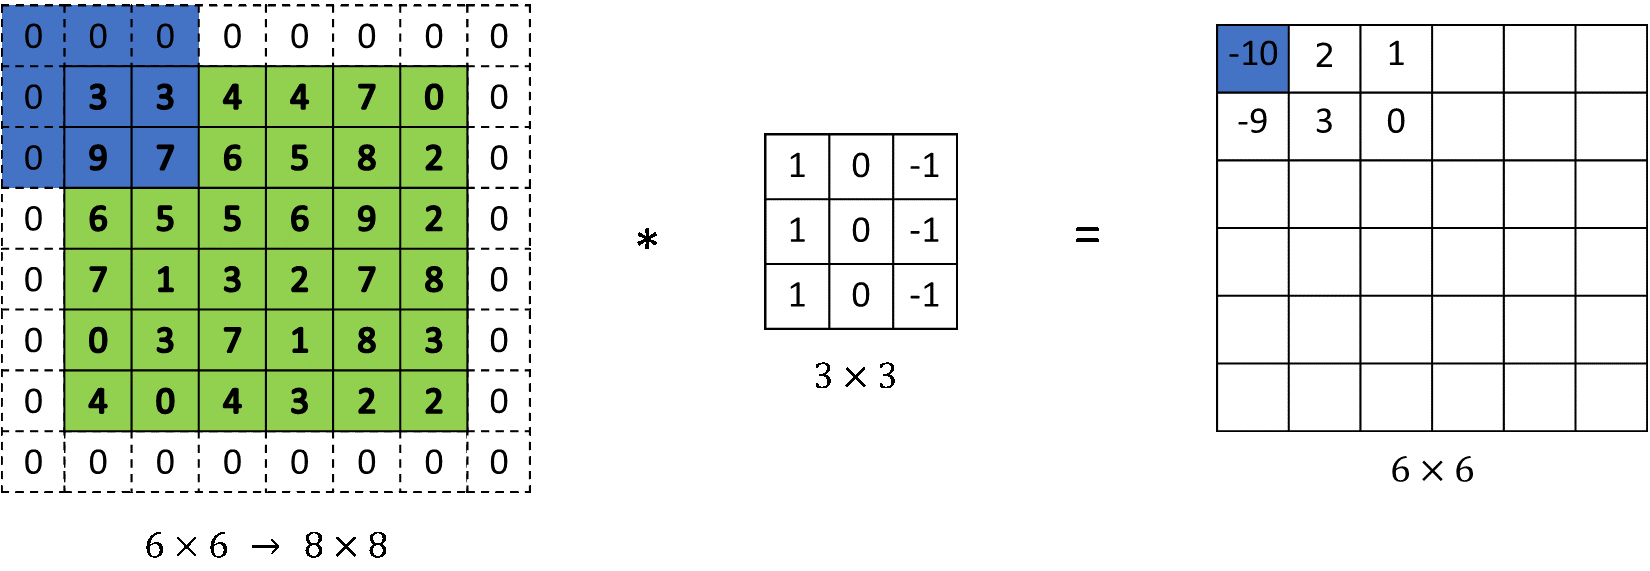
\includegraphics[width=0.9\columnwidth]{images/Padding3.png}
        \caption{\hyperlink{https://datahacker.rs/what-is-padding-cnn/}{DataHacker.rs: CNN Padding - }Applying padding of 1 before convolving with $3 \times 3$ filter}
        % \label{fig:my_label}
    \end{figure}
\end{center}
}

%%%%%%%%%%%%%%%%%%%%%%%%%%%%%%%%%%%%%%%%%%%%%%%%%%%%%%%%%%%%%%%%%%%%%%%%%%%%%%%%%%%%%%%%%%%%%%%
\frame{\frametitle{Padding}
\begin{center}
    \begin{itemize}
        \item\color{red}\large{It is common to use $P = (F - 1) / 2$ with stride 1 to preserve the input size.}
    \end{itemize}
    \begin{figure}
        \centering
        \includesvg[width=0.4\columnwidth]{images/Padding4.svg}
        \caption{Applying zero-padding to a 7x7 input with padding 1}
        % \label{fig:my_label}
    \end{figure}
\end{center}
}

%%%%%%%%%%%%%%%%%%%%%%%%%%%%%%%%%%%%%%%%%%%%%%%%%%%%%%%%%%%%%%%%%%%%%%%%%%%%%%%%%%%%%%%%%%%%%%%
\frame{\frametitle{Padding}
\begin{center}
    \begin{itemize}
        \item\large{It is common to use $P = (F - 1) / 2$ with stride 1 to preserve the input size.}
        \item\color{red}\large{$OutputSize = (N + 2P - F) / Stride + 1$}
        \end{itemize}
    \begin{figure}
        \centering
        \includesvg[width=0.4\columnwidth]{images/Padding4.svg}
        \caption{Applying zero-padding to a 7x7 input with padding 1}
        % \label{fig:my_label}
    \end{figure}
\end{center}
}

%%%%%%%%%%%%%%%%%%%%%%%%%%%%%%%%%%%%%%%%%%%%%%%%%%%%%%%%%%%%%%%%%%%%%%%%%%%%%%%%%%%%%%%%%%%%%%%
\frame{\frametitle{Padding}
\begin{center}
    \begin{itemize}
        \item\large{It is common to use $P = (F - 1) / 2$ with stride 1 to preserve the input size.}
        \item\large{$OutputSize = (N + 2P - F) / Stride + 1$}
        \newline
    \end{itemize}
    \begin{minipage}{0.5\textwidth}
        \begin{figure}
            \centering
            \includesvg[width=0.7\columnwidth]{images/Padding4.svg}
            \caption{Applying zero-padding to a 7x7 input with padding 1}
        \end{figure}

    \end{minipage} \hfill
    \begin{minipage}{0.45\textwidth}
        \large{\color{red}7x7 input, stride 1, P to preserve the dimentions?}
        \begin{itemize}
            \item $F = 3 --> P = 1$
            \item $F = 5 --> P = 2$
            \item $F = 7 --> P = 3$
        \end{itemize}
    \end{minipage}
    
\end{center}
}
%%%%%%%%%%%%%%%%%%%%%%%%%%%%%%%%%%%%%%%%%%%%%%%%%%%%%%%%%%%%%%%%%%%%%%%%%%%%%%%%%%%%%%%%%%%%%%%
\section{Pooling}
%%%%%%%%%%%%%%%%%%%%%%%%%%%%%%%%%%%%%%%%%%%%%%%%%%%%%%%%%%%%%%%%%%%%%%%%%%%%%%%%%%%%%%%%%%%%%%%
\frame{\frametitle{Pooling}
\begin{itemize}
        \item{Pooling is performed in neural networks to reduce variance and computation complexity}
\end{itemize}
\begin{center}
    \begin{figure}
        \centering
        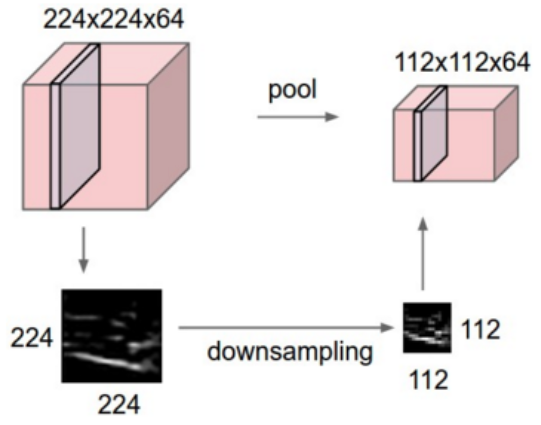
\includegraphics[width=0.4\columnwidth]{images/Pooling_1.png}
        \caption{Pooling Layer}
        % \label{fig:testtt}
    \end{figure}
\end{center}
}
%%%%%%%%%%%%%%%%%%%%%%%%%%%%%%%%%%%%%%%%%%%%%%%%%%%%%%%%%%%%%%%%%%%%%%%%%%%%%%%%%%%%%%%%%%%%%%%
\frame{\frametitle{Pooling: How It Works}
\begin{itemize}
    \item Pooling layers aggregate the
inputs using an aggregation function such as the max or mean.
\end{itemize}
\begin{center}
    \begin{figure}
        \centering
        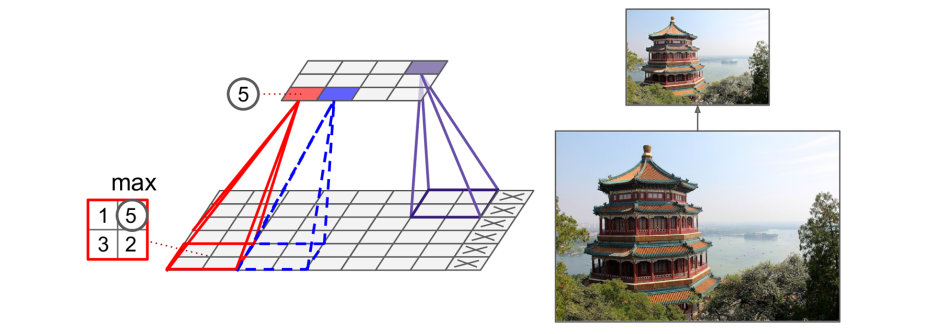
\includegraphics[width=0.9\columnwidth]{images/Pooling_2.png}
        \caption{Max pooling layer (2 × 2 pooling kernel, stride 2, no padding)}
        % \label{fig:testtt}
    \end{figure}
\end{center}
}

%%%%%%%%%%%%%%%%%%%%%%%%%%%%%%%%%%%%%%%%%%%%%%%%%%%%%%%%%%%%%%%%%%%%%%%%%%%%%%%%%%%%%%%%%%%%%%%
\frame{\frametitle{Pooling: Benefits}
\begin{itemize}
        \item{A Pooling layer's goal is to sub-sample the input in order to reduce:}
        \begin{itemize}
            \item The computational load
            \item The memory usage
            \item The number of parameters
            \item Limiting the risk of overfitting
        \end{itemize}
\end{itemize}
}
%%%%%%%%%%%%%%%%%%%%%%%%%%%%%%%%%%%%%%%%%%%%%%%%%%%%%%%%%%%%%%%%%%%%%%%%%%%%%%%%%%%%%%%%%%%%%%%
\frame{\frametitle{Pooling: Types}
\begin{itemize}
    \item Max Pooling: gives better results when the background is white and the object is dark
    \item Min Pooling: gives better results when the background is dark and the object is white
    \item Average Pooling: smoothes the picture
\end{itemize}
\begin{center}
    \begin{figure}
        \centering
        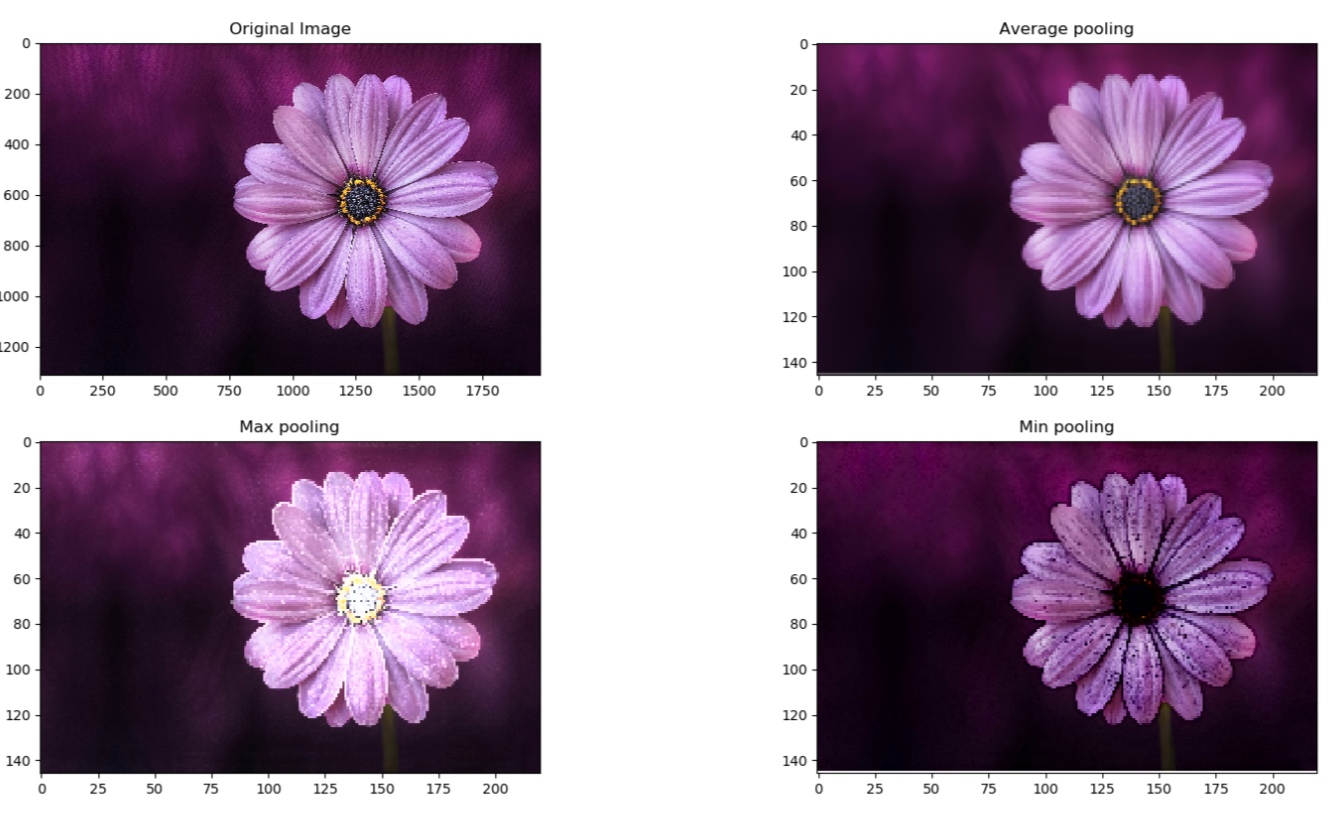
\includegraphics[width=0.7\columnwidth]{images/Pooling_3.png}
        \caption{Effects of different pooling layers}
        % \label{fig:testtt}
    \end{figure}
\end{center}
}
%%%%%%%%%%%%%%%%%%%%%%%%%%%%%%%%%%%%%%%%%%%%%%%%%%%%%%%%%%%%%%%%%%%%%%%%%%%%%%%%%%%%%%%%%%%%%%%
\frame{\frametitle{Pooling: Max Pooling}
\begin{itemize}
    \item Most common type of pooling layer
    \item Invariance to small translations
\end{itemize}
\begin{center}
    \begin{figure}
        \centering
        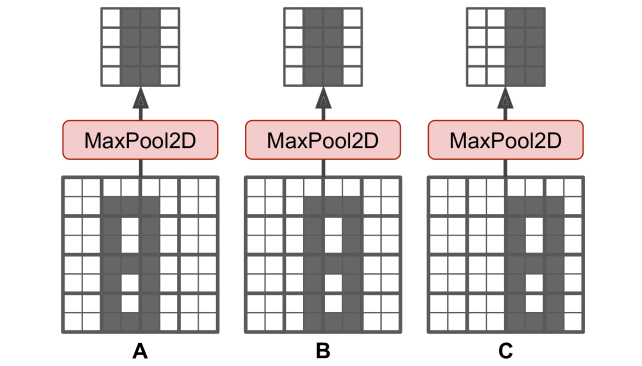
\includegraphics[width=0.8\columnwidth]{images/Pooling_4.png}
        \caption{Invariance to small translations}
        % \label{fig:testtt}
    \end{figure}
\end{center}
}
%%%%%%%%%%%%%%%%%%%%%%%%%%%%%%%%%%%%%%%%%%%%%%%%%%%%%%%%%%%%%%%%%%%%%%%%%%%%%%%%%%%%%%%%%%%%%%%
\section{Dilation}
%%%%%%%%%%%%%%%%%%%%%%%%%%%%%%%%%%%%%%%%%%%%%%%%%%%%%%%%%%%%%%%%%%%%%%%%%%%%%%%%%%%%%%%%%%%%%%%
\frame{\frametitle{Dilation}
\begin{itemize}
        \item{It expands the kernel (input) by inserting spaces between its consecutive elements}
\end{itemize}
\begin{center}
    \begin{figure}
        \centering
        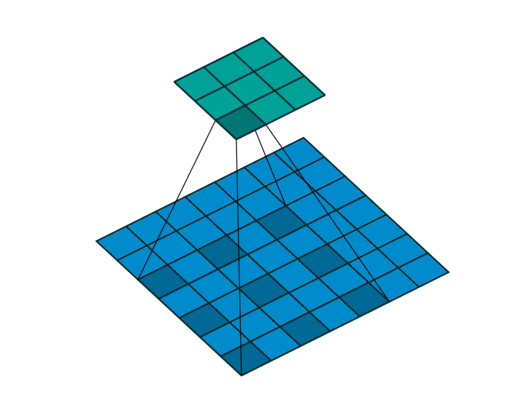
\includegraphics[width=0.25\columnwidth]{images/Dilated_1.png}
        % \caption{Standard Convolution (l=1)}
        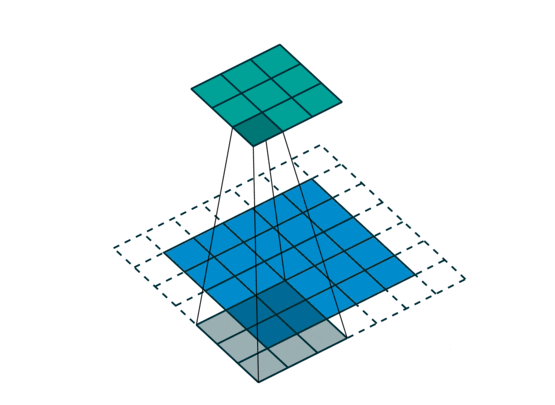
\includegraphics[width=0.27\columnwidth]{images/Dilated_2.png}
        \caption{Dilated Convolution \((l=2)\) vs. Standard Convolution \((l=1)\)}
        % \label{fig:testtt}
    \end{figure}
\end{center}
}
%%%%%%%%%%%%%%%%%%%%%%%%%%%%%%%%%%%%%%%%%%%%%%%%%%%%%%%%%%%%%%%%%%%%%%%%%%%%%%%%%%%%%%%%%%%%%%%
\frame{\frametitle{Dilation: Benefits}
\begin{itemize}
        \item Since dilated convolutions support exponential expansion in the context of the receptive field, there is no loss of resolution.
        \item Dilated convolutions use 'l' as the parameter for the dilation rate. As we increase the value of 'l' it allows one to have a larger receptive field which is really helpful as we are able to view more data points thus saving computation and memory costs
\end{itemize}
\begin{center}
    \begin{figure}
        \centering
        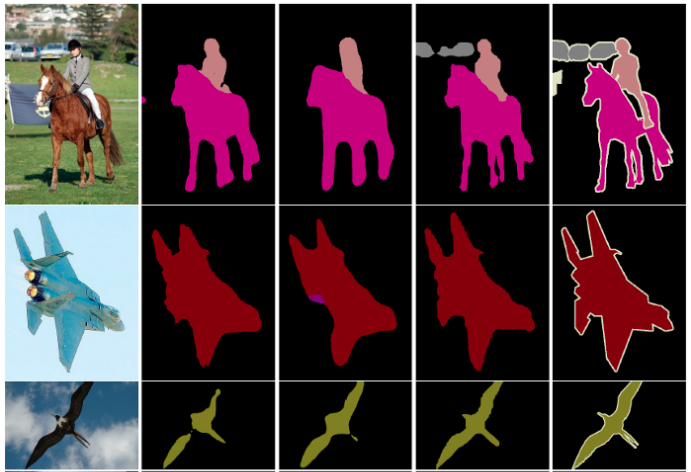
\includegraphics[width=0.5\columnwidth]{images/Dilated_3.png}
        \caption{Image - FCN-8s - DeepLab - DilatedNet - Ground Truth}
        % \label{fig:testtt}
    \end{figure}
\end{center}
}

%%%%%%%%%%%%%%%%%%%%%%%%%%%%%%%%%%%%%%%%%%%%%%%%%%%%%%%%%%%%%%%%%%%%%%%%%%%%%%%%%%%%%%%%%%%%%%%
\section{Channels}
%%%%%%%%%%%%%%%%%%%%%%%%%%%%%%%%%%%%%%%%%%%%%%%%%%%%%%%%%%%%%%%%%%%%%%%%%%%%%%%%%%%%%%%%%%%%%%%
\frame{\frametitle{Channels}
So far, we have talked about 2D inputs, but although images are 2D, we need to represent them as 3D matrices to show their colors:
\newline
\begin{itemize}
    \item Pixel values range from \tc{keywords}{0 to 255}
    \item We cannot represent all the colors in a picture with only one channel of numbers from 0 to 255
\end{itemize}
\begin{center}
    \begin{figure}
        \centering
        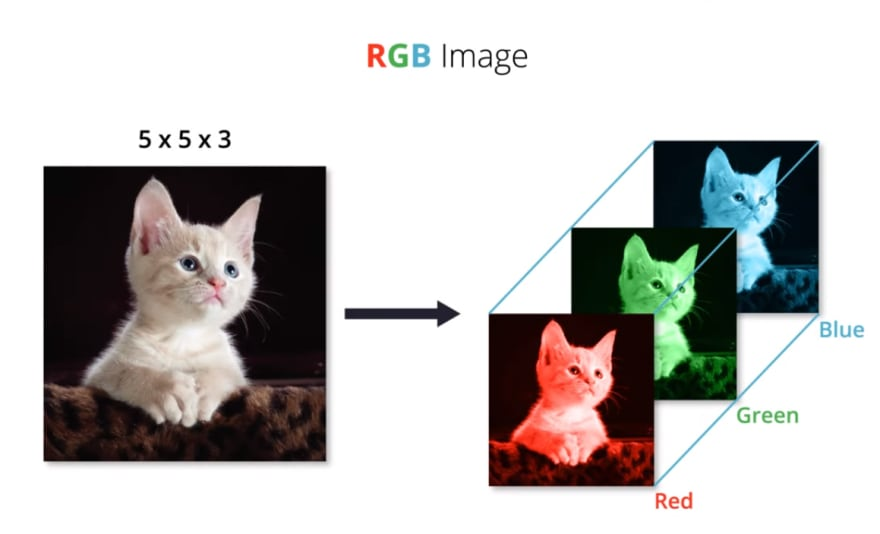
\includegraphics[width=0.7\columnwidth]{images/channels1.jpeg}
        \caption{RGB Image, \href{https://dev.to/sandeepbalachandran/machine-learning-going-furthur-with-cnn-part-2-41km}{Source}}
    \end{figure}
\end{center}
}
%%%%%%%%%%%%%%%%%%%%%%%%%%%%%%%%%%%%%%%%%%%%%%%%%%%%%%%%%%%%%%%%%%%%%%%%%%%%%%%%%%%%%%%%%%%%%%%
\frame{\frametitle{Channels}
So far, we have talked about 2D inputs, but although images are 2D, we need to represent them as 3D matrices to show their colors:
\newline
\begin{itemize}
    \item \tc{keywords}{So we represent them in 3 channels}
    \item They consist of 3 channels: Red, Green and Blue (RGB images)
    \item Shape: (height x width x 3)
\end{itemize}
\begin{center}
    \begin{figure}
        \centering
        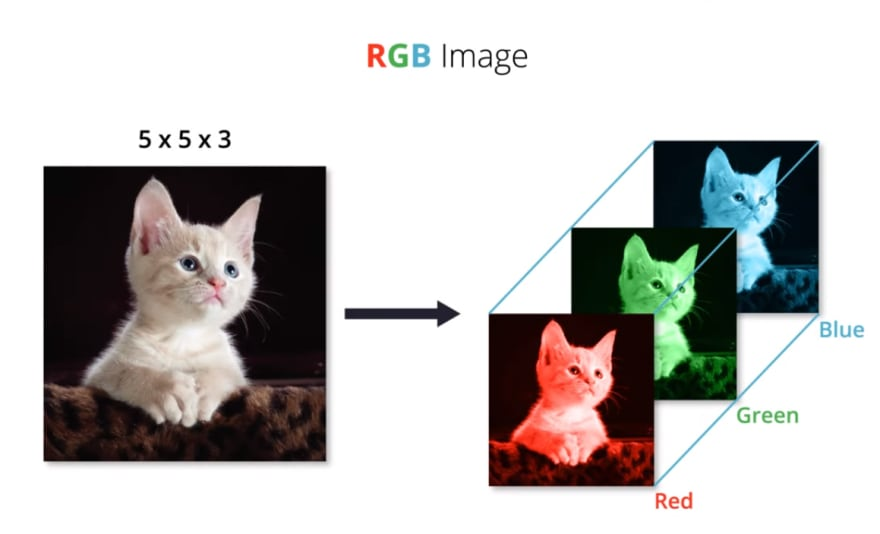
\includegraphics[width=0.7\columnwidth]{images/channels1.jpeg}
        \caption{RGB Image, \href{https://dev.to/sandeepbalachandran/machine-learning-going-furthur-with-cnn-part-2-41km}{Source}}
    \end{figure}
\end{center}

}

%%%%%%%%%%%%%%%%%%%%%%%%%%%%%%%%%%%%%%%%%%%%%%%%%%%%%%%%%%%%%%%%%%%%%%%%%%%%%%%%%%%%%%%%%%%%%%%
\frame{\frametitle{Channels}
So far, we have talked about 2D inputs, but although images are 2D, we need to represent them as 3D matrices to show their colors:
\newline
\begin{itemize}
    \item They consist of 3 channels: Red, Green and Blue (RGB images)
    \item Shape: (height x width x 3)
\end{itemize}
\begin{center}
    \begin{figure}
        \centering
        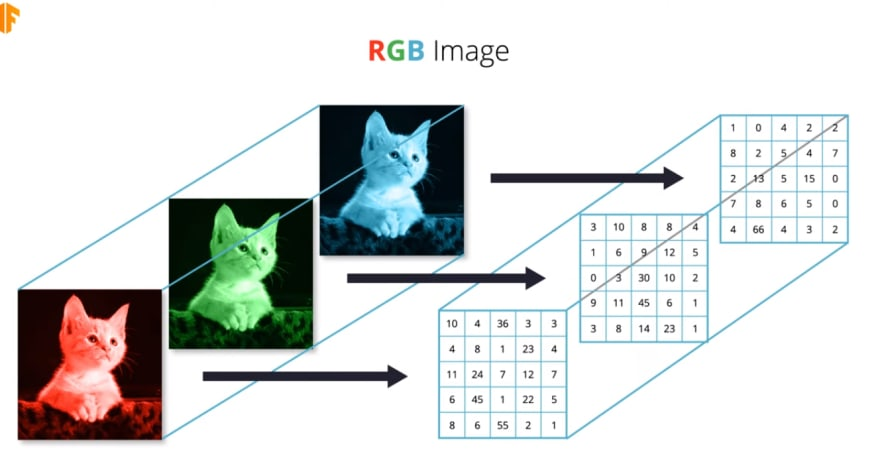
\includegraphics[width=0.7\columnwidth]{images/channels2.jpeg}
        \caption{RGB Image, \href{https://dev.to/sandeepbalachandran/machine-learning-going-furthur-with-cnn-part-2-41km}{Source}}
    \end{figure}
\end{center}

}

%%%%%%%%%%%%%%%%%%%%%%%%%%%%%%%%%%%%%%%%%%%%%%%%%%%%%%%%%%%%%%%%%%%%%%%%%%%%%%%%%%%%%%%%%%%%%%%
\frame{\frametitle{Channels}
So far, we have talked about 2D inputs, but although images are 2D, we need to represent them as 3D matrices to show their colors:
\newline
\begin{itemize}
    \item They consist of 3 channels: Red, Green and Blue (RGB images)
    \item Shape: (height x width x 3)
\end{itemize}
\begin{center}
    \begin{figure}
        \centering
        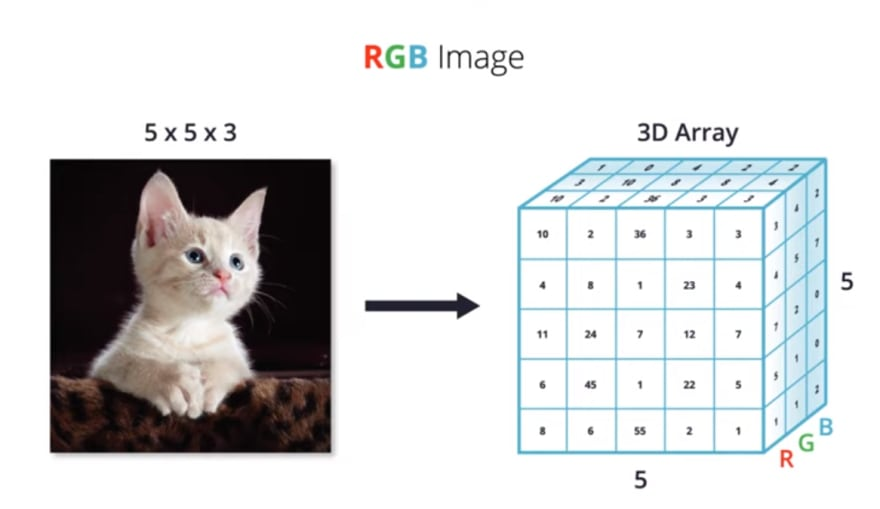
\includegraphics[width=0.7\columnwidth]{images/channels3.jpeg}
        \caption{RGB Image, \href{https://dev.to/sandeepbalachandran/machine-learning-going-furthur-with-cnn-part-2-41km}{Source}}
    \end{figure}
\end{center}
}
%%%%%%%%%%%%%%%%%%%%%%%%%%%%%%%%%%%%%%%%%%%%%%%%%%%%%%%%%%%%%%%%%%%%%%%%%%%%%%%%%%%%%%%%%%%%%%%
\frame{\frametitle{Channels}
- As said before: "Filters always extend the full depth of the input. \newline(\#Input channels == \#Filter Channels)"
\begin{center}
    \begin{figure}
        \centering
        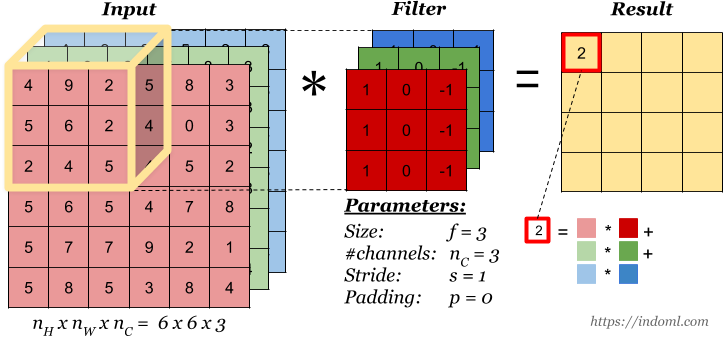
\includegraphics[width=0.7\columnwidth]{images/channels4.png}
        \caption{The total number of multiplications to calculate the result is (4 x 4) x (3 x 3 x 3) = 432, \href{https://indoml.com/2018/03/07/student-notes-convolutional-neural-networks-cnn-introduction/}{Source}}
    \end{figure}
\end{center}
}
%%%%%%%%%%%%%%%%%%%%%%%%%%%%%%%%%%%%%%%%%%%%%%%%%%%%%%%%%%%%%%%%%%%%%%%%%%%%%%%%%%%%%%%%%%%%%%%

\frame{\frametitle{Channels}
- As said before: "Filters always extend the full depth of the input volume. (\#Input channels == \#Filter Channels)"
\newline
\color{red}- Each filter results in one output channel. We can apply multiple different filters to obtain multiple output channels. Each channel can learn something distinct.

\begin{center}
    \begin{figure}
        \centering
        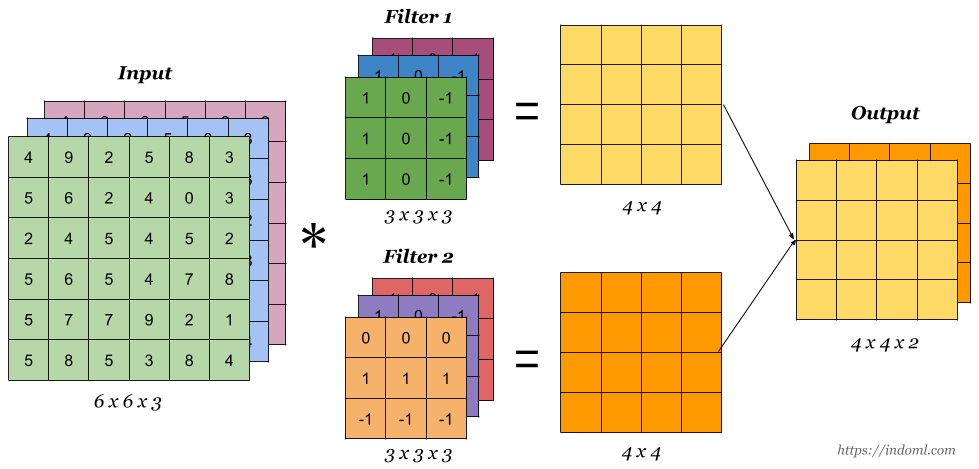
\includegraphics[width=0.7\columnwidth]{images/channels5.png}
        \caption{The total number of multiplications to calculate the result is (4 x 4 x 2) x (3 x 3 x 3) = 864, \href{https://indoml.com/2018/03/07/student-notes-convolutional-neural-networks-cnn-introduction/}{Source}}
    \end{figure}
\end{center}
}


%%%%%%%%%%%%%%%%%%%%%%%%%%%%%%%%%%%%%%%%%%%%%%%%%%%%%%%%%%%%%%%%%%%%%%%%%%%%%%%%%%%%%%%%%%%%%%%

\foreach \i in {1,...,18}
{
    \frame{\frametitle{Channels}
    \normalsize
    Let's have a closer look to how the calculations with more than one filter work:

    \begin{figure}
    \centering
        \includegraphics[width=0.55\columnwidth]{images/cs231n-conv-\i.png}
        \caption{Great Visualization by CS231n, \href{https://cs231n.github.io/convolutional-networks/}{Source}}
    \end{figure}
    }
}
%%%%%%%%%%%%%%%%%%%%%%%%%%%%%%%%%%%%%%%%%%%%%%%%%%%%%%%%%%%%%%%%%%%%%%%%%%%%%%%%%%%%%%%%%%%%%%%

\frame{\frametitle{Channels}
\color{red}- We apply several filters and stack the output together to get a multilayer output, with each layer representing something it learned.
\begin{center}
    \begin{figure}
        \centering
        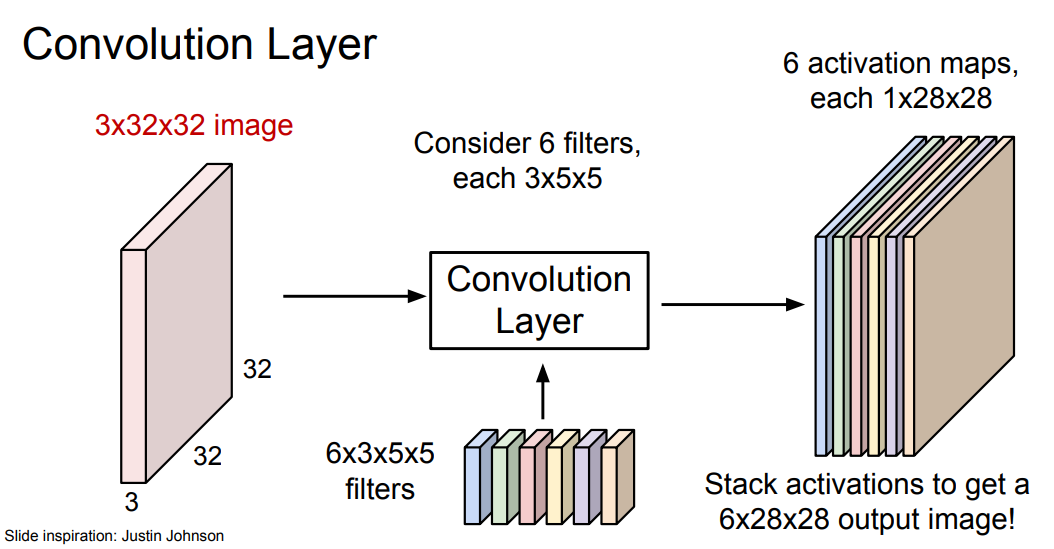
\includegraphics[width=0.8\columnwidth]{images/channels6.png}
        \caption{\href{http://cs231n.stanford.edu/slides/2022/lecture_5_ruohan.pdf}{Slide from CS231n}}
    \end{figure}
\end{center}
}

%%%%%%%%%%%%%%%%%%%%%%%%%%%%%%%%%%%%%%%%%%%%%%%%%%%%%%%%%%%%%%%%%%%%%%%%%%%%%%%%%%%%%%%%%%%%%%%

\frame{\frametitle{Channels}
- We apply several filters and stack the output together to get a multilayer output, with each layer representing something it learned.
\newline
\color{red}- Some kernels learn to recognize vertical lines, some circles, and some, specific objects:
\begin{center}
    \begin{figure}
        \centering
        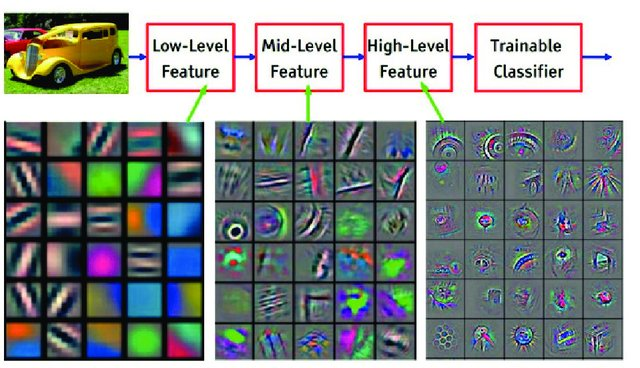
\includegraphics[width=0.7\columnwidth]{images/channels7.jpg}
        \caption{Each kernel learning something different, \href{https://www.researchgate.net/publication/318967374_En_ny_aera_for_uthenting_av_informasjon_fra_satellittbilder_ved_hjelp_av_maskinlaering_Mathilde_Orstavik_og_Terje_Midtbo_Mathilde_Orstavik_and_Terje_Midtbo_A_New_Era_for_Feature_Extraction_in_Remotely}{Source}}
    \end{figure}
\end{center}
}
%%%%%%%%%%%%%%%%%%%%%%%%%%%%%%%%%%%%%%%%%%%%%%%%%%%%%%%%%%%%%%%%%%%%%%%%%%%%%%%%%%%%%%%%%%%%%%%
\section{Arithmetic of CNNs}
%%%%%%%%%%%%%%%%%%%%%%%%%%%%%%%%%%%%%%%%%%%%%%%%%%%%%%%%%%%%%%%%%%%%%%%%%%%%%%%%%%%%%%%%%%%%%%%
    \frame{\frametitle{Arithmetic of CNNs}
We will focus on the following simplified setting:
\begin{itemize}
        \item 2-D discrete convolutions \((N = 2)\)
        \item Square inputs \((i_1 = i_2 = i)\)
        \item Square kernel size \((k_1 = k_2 = k)\)
        \item Same strides along both axes \((s_1 = s_2 = s)\)
        \item Same zero padding along both axes \((p_1 = p_2 = p)\)
\end{itemize}
}
%%%%%%%%%%%%%%%%%%%%%%%%%%%%%%%%%%%%%%%%%%%%%%%%%%%%%%%%%%%%%%%%%%%%%%%%%%%%%%%%%%%%%%%%%%%%%%%
\frame{\frametitle{Arithmetic of CNNs: No zero padding, unit strides}
\begin{itemize}
        \item For any \(i\) and \(k\), and for \(s = 1\) and \(p = 0\):
\end{itemize}

\begin{center}
\begin{equation}
\begin{split}
o = (i - k) + 1 
\end{split}
\end{equation}
\end{center}

\begin{center}
    \begin{figure}
        \centering
        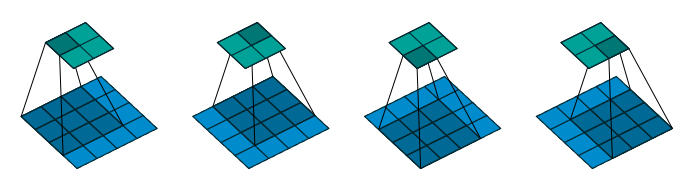
\includegraphics[width=0.7\columnwidth]{images/Arithmetic_1.png}
        \caption{Convolving a 3 × 3 kernel over a 4 × 4
input using unit strides (i.e., i = 4, k = 3, s = 1 and p = 0)}
    \end{figure}
\end{center}
}

%%%%%%%%%%%%%%%%%%%%%%%%%%%%%%%%%%%%%%%%%%%%%%%%%%%%%%%%%%%%%%%%%%%%%%%%%%%%%%%%%%%%%%%%%%%%%%%
\frame{\frametitle{Arithmetic of CNNs: Zero padding, unit strides}
\begin{itemize}
        \item For any \(i\), \(k\) and \(p\), and for \(s = 1\):
\end{itemize}

\begin{center}
\begin{equation}
\begin{split}
o = (i - k) + 2p + 1  \newline
\end{split}
\end{equation}
\end{center}

\begin{center}
    \begin{figure}
        \centering
        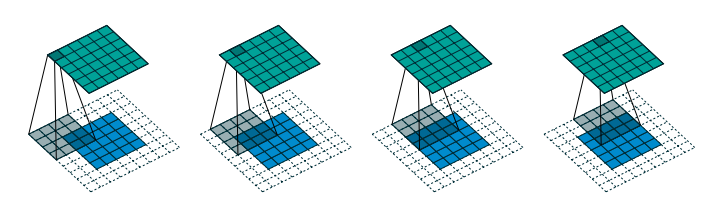
\includegraphics[width=0.7\columnwidth]{images/Arithmetic_2.png}
        \caption{Convolving a 4 × 4 kernel over a
5 × 5 input padded with a 2 × 2 border of zeros using unit strides (i.e., i = 5,
k = 4, s = 1 and p = 2)}
    \end{figure}
\end{center}
}
%%%%%%%%%%%%%%%%%%%%%%%%%%%%%%%%%%%%%%%%%%%%%%%%%%%%%%%%%%%%%%%%%%%%%%%%%%%%%%%%%%%%%%%%%%%%%%%
\frame{\frametitle{Arithmetic of CNNs: Half (same) padding}
\begin{itemize}
        \item For any \(i\) and for\(k\) odd (\(k = 2n + 1, n \in \mathbb{N}\)), \(s=1\) and \(p = ⌊k/2⌋ = n\):
\end{itemize}

\begin{center}
\begin{equation}
\begin{split}
o & =  i + 2⌊k/2⌋ - (k-1) \newline
& = i + 2n - 2n \newline
& = i
\end{split}
\end{equation}
\end{center}

\begin{center}
    \begin{figure}
        \centering
        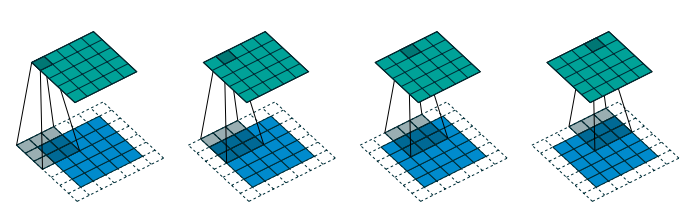
\includegraphics[width=0.7\columnwidth]{images/Arithmetic_3.png}
        \caption{Convolving a 3 × 3 kernel over a 5 × 5
input using half padding and unit strides (i.e., i = 5, k = 3, s = 1 and p = 1)}
    \end{figure}
\end{center}
}
%%%%%%%%%%%%%%%%%%%%%%%%%%%%%%%%%%%%%%%%%%%%%%%%%%%%%%%%%%%%%%%%%%%%%%%%%%%%%%%%%%%%%%%%%%%%%%%
\frame{\frametitle{Arithmetic of CNNs: Full padding}
\begin{itemize}
        \item For any \(i\) and \(k\), and for \(p = k − 1\) and \(s = 1\):
\end{itemize}

\begin{center}
\begin{equation}
\begin{split}
o & = i + 2(k-1) - (k-1) \newline
& = i + 2(k-1
\end{split}
\end{equation}
\end{center}

\begin{center}
    \begin{figure}
        \centering
        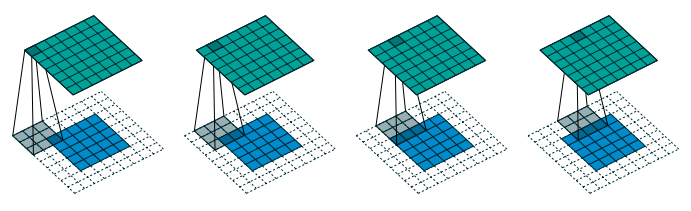
\includegraphics[width=0.7\columnwidth]{images/Arithmetic_4.png}
        \caption{Convolving a 3 × 3 kernel over a 5 × 5
input using full padding and unit strides (i.e., i = 5, k = 3, s = 1 and p = 2)}
    \end{figure}
\end{center}
}
%%%%%%%%%%%%%%%%%%%%%%%%%%%%%%%%%%%%%%%%%%%%%%%%%%%%%%%%%%%%%%%%%%%%%%%%%%%%%%%%%%%%%%%%%%%%%%%
\frame{\frametitle{Arithmetic of CNNs: No zero padding, non-unit strides}
\begin{itemize}
        \item For any \(i\), \(k\) and \(s\), and for \(p = 0\):
\end{itemize}

\begin{center}
\begin{equation}
\begin{split}
o= ⌊\frac{i-k} {s}⌋ + 1
\end{split}
\end{equation}
\end{center}

\begin{center}
    \begin{figure}
        \centering
        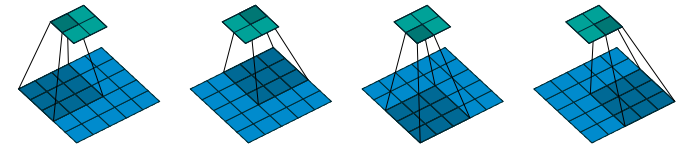
\includegraphics[width=0.7\columnwidth]{images/Arithmetic_5.png}
        \caption{Convolving a 3 × 3 kernel over
a 5 × 5 input using 2 × 2 strides (i.e., i = 5, k = 3, s = 2 and p = 0)}
    \end{figure}
\end{center}
}
%%%%%%%%%%%%%%%%%%%%%%%%%%%%%%%%%%%%%%%%%%%%%%%%%%%%%%%%%%%%%%%%%%%%%%%%%%%%%%%%%%%%%%%%%%%%%%%
\frame{\frametitle{Arithmetic of CNNs: Zero padding, non-unit strides}
\begin{itemize}
        \item For any \(i\), \(k\) and \(s\), and for \(p = 0\):
\end{itemize}

\begin{center}
\begin{equation}
\begin{split}
o= ⌊\frac{i+2p-k} {s}⌋ + 1
\end{split}
\end{equation}
\end{center}

\begin{center}
    \begin{figure}
        \centering
        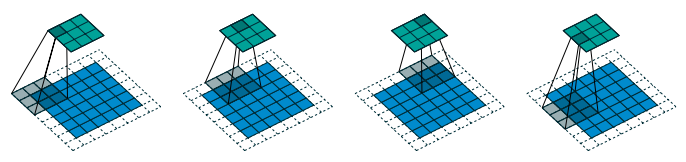
\includegraphics[width=0.7\columnwidth]{images/Arithmetic_6.png}
        \caption{Convolving a 3 × 3 kernel over a
6 × 6 input padded with a 1 × 1 border of zeros using 2 × 2 strides (i.e., i = 6,
k = 3, s = 2 and p = 1). In this case, the bottom row and right column of the
zero-padded input are not covered by the kernel}
    \end{figure}
\end{center}
}

%%%%%%%%%%%%%%%%%%%%%%%%%%%%%%%%%%%%%%%%%%%%%%%%%%%%%%%%%%%%%%%%%%%%%%%%%%%%%%%%%%%%%%%%%%%%%%%

\section{Upsample CNN}
%%%%%%%%%%%%%%%%%%%%%%%%%%%%%%%%%%%%%%%%%%%%%%%%%%%%%%%%%%%%%%%%%%%%%%%%%%%%%%%%%%%%%%%%%%%%%%%
\frame{\frametitle{Upsample CNN}
\begin{itemize}
        \item Resizing feature maps is a common operation in many neural networks, especially those that perform some kind of image segmentation task
        \item This kind of architecture is famously known as the Encoder-Decoder network
\end{itemize}
\begin{center}
    \begin{figure}
        \centering
        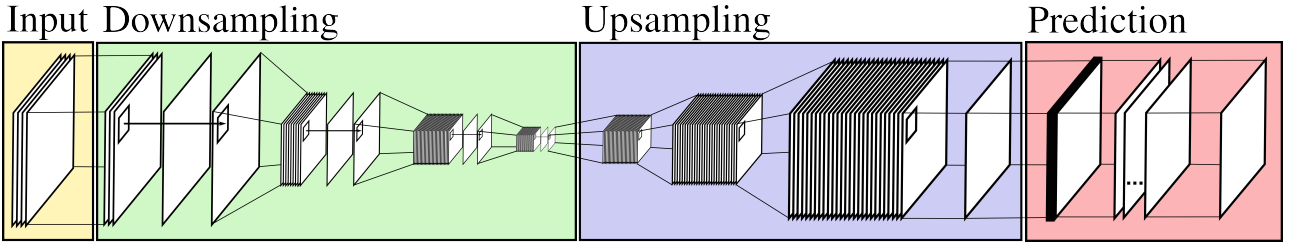
\includegraphics[width=0.7\columnwidth]{images/Upsamlpe_0.png}
        \caption{Schematic of the Downsampling and Upsampling}
    \end{figure}
\end{center}
}
%%%%%%%%%%%%%%%%%%%%%%%%%%%%%%%%%%%%%%%%%%%%%%%%%%%%%%%%%%%%%%%%%%%%%%%%%%%%%%%%%%%%%%%%%%%%%%%
\frame{\frametitle{Upsample CNN: Techniques}
\begin{itemize}
        \item 1- Nearest Neighbors: In Nearest Neighbors, as the name suggests, we take an input pixel value and copy it to the K-Nearest Neighbors, where K depends on the expected output.
\end{itemize}

\begin{center}
    \begin{figure}
        \centering
        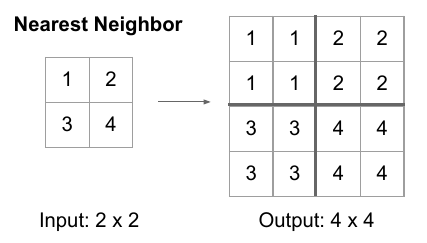
\includegraphics[width=0.4\columnwidth]{images/Upsamlpe_1.png}
        \caption{Nearest Neighbors Upsampling}
    \end{figure}
\end{center}
}
%%%%%%%%%%%%%%%%%%%%%%%%%%%%%%%%%%%%%%%%%%%%%%%%%%%%%%%%%%%%%%%%%%%%%%%%%%%%%%%%%%%%%%%%%%%%%%%
\frame{\frametitle{Upsample CNN: Techniques}
\begin{itemize}
        \item 2- Bi-Linear Interpolation: In Bi-Linear Interpolation, we take the 4 nearest pixel value of the input pixel and perform a weighted average based on the distance of the four nearest cells smoothing the output
\end{itemize}

\begin{center}
    \begin{figure}
        \centering
        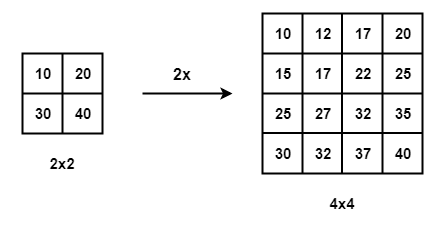
\includegraphics[width=0.4\columnwidth]{images/Upsamlpe_2.png}
        \caption{Bi-Linear Interpolation}
    \end{figure}
\end{center}
}
%%%%%%%%%%%%%%%%%%%%%%%%%%%%%%%%%%%%%%%%%%%%%%%%%%%%%%%%%%%%%%%%%%%%%%%%%%%%%%%%%%%%%%%%%%%%%%%
\frame{\frametitle{Upsample CNN: Techniques}
\begin{itemize}
        \item 3- Bed Of Nails: In Bed of Nails, we copy the value of the input pixel at the corresponding position in the output image and filling zeros in the remaining positions.
\end{itemize}

\begin{center}
    \begin{figure}
        \centering
        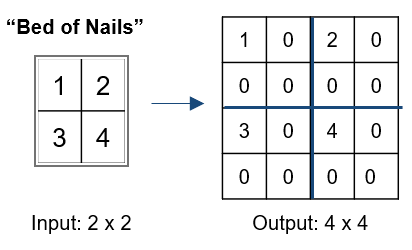
\includegraphics[width=0.4\columnwidth]{images/Upsamlpe_3.png}
        \caption{Bed of Nails Upsampling}
    \end{figure}
\end{center}
}
%%%%%%%%%%%%%%%%%%%%%%%%%%%%%%%%%%%%%%%%%%%%%%%%%%%%%%%%%%%%%%%%%%%%%%%%%%%%%%%%%%%%%%%%%%%%%%%
\frame{\frametitle{Upsample CNN: Techniques}
\begin{itemize}
        \item 4- Max-Unpooling: To perform max-unpooling, first, the index of the maximum value is saved for every max-pooling layer during the encoding step. The saved index is then used during the Decoding step where the input pixel is mapped to the saved index, filling zeros everywhere else
\end{itemize}

\begin{center}
    \begin{figure}
        \centering
        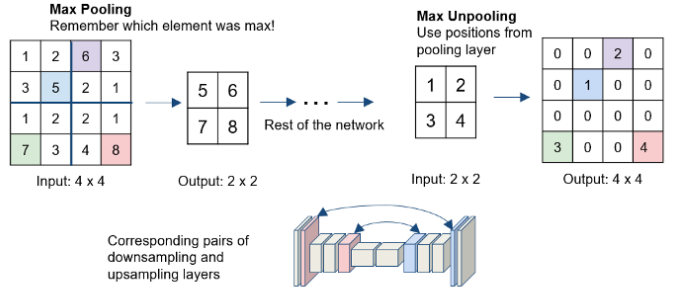
\includegraphics[width=0.7\columnwidth]{images/Upsamlpe_4.png}
        \caption{Max-Unpooling Upsampling}
    \end{figure}
\end{center}
}
%%%%%%%%%%%%%%%%%%%%%%%%%%%%%%%%%%%%%%%%%%%%%%%%%%%%%%%%%%%%%%%%%%%%%%%%%%%%%%%%%%%%%%%%%%%%%%%

\section{Transposed CNN}
%%%%%%%%%%%%%%%%%%%%%%%%%%%%%%%%%%%%%%%%%%%%%%%%%%%%%%%%%%%%%%%%%%%%%%%%%%%%%%%%%%%%%%%%%%%%%%%
\frame{\frametitle{Transposed CNN}
\begin{itemize}
        \item Transposed Convolutions are used to upsample the input feature map to a desired output feature map using some learnable parameters
        \item They are the backbone of the modern segmentation and super-resolution algorithms
        \item They provide the best and most generalized upsampling of abstract representations
\end{itemize}
\begin{center}
    \begin{figure}
        \centering
        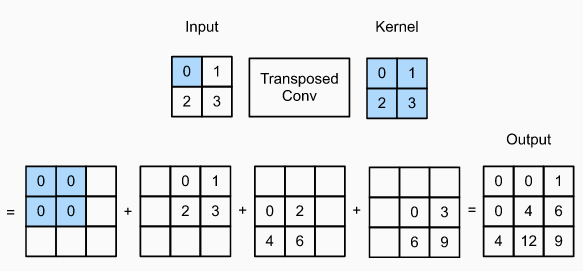
\includegraphics[width=0.7\columnwidth]{images/Transposed_1.png}
        \caption{Transposed convolution with a \(2 \times 2\)  kernel. The shaded portions are a portion of an intermediate tensor as well as the input and kernel tensor elements used for the computation.}
    \end{figure}
\end{center}
}
%%%%%%%%%%%%%%%%%%%%%%%%%%%%%%%%%%%%%%%%%%%%%%%%%%%%%%%%%%%%%%%%%%%%%%%%%%%%%%%%%%%%%%%%%%%%%%%
\frame{\frametitle{Transposed CNN: Problem}
\begin{itemize}
        \item Transposed convolutions suffer from chequered board effects as shown below. The main cause of this is uneven overlap at some parts of the image causing artifacts. This can be fixed or reduced by using kernel-size divisible by the stride, for e.g taking a kernel size of \(2 \times 2\) or \(4 \times 4\) when having a stride of 2.

\end{itemize}
\begin{center}
    \begin{figure}
        \centering
        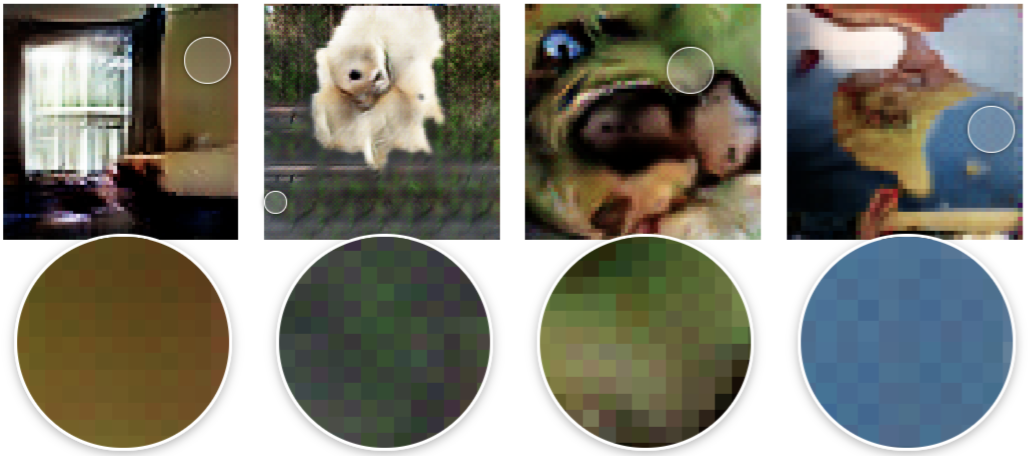
\includegraphics[width=0.7\columnwidth]{images/Transposed_2.png}
        \caption{Checkerboard artifacts effect}
    \end{figure}
\end{center}
}


%%%%%%%%%%%%%%%%%%%%%%%%%%%%%%%%%%%%%%%%%%%%%%%%%%%%%%%%%%%%%%%%%%%%%%%%%%%%%%%%%%%%%%%%%%%%%%%
\frame{\frametitle{Final Notes}
\centering
\vspace{50 pt}
\textbf{Thank You!}
\vspace{50pt}

\textbf{Any Question?}
}
%%%%%%%%%%%%%%%%%%%%%%%%%%%%%%%%%%%%%%%%%%%%%%%%%%%%%%%%%%%%%%%%%%%%%%%%%%%%%%%%%%%%%%%%%%%%%%%
\frame{\frametitle{Refrences}
\begin{itemize}
    \item Hands-On Machine Learning with Scikit-Learn, Keras, and TensorFlow - Aurélien Géron - 2019 - \hyperlink{https://www.amazon.de/-/en/Aurélien-Géron/dp/1492032646}{Link}
    \item Deep Learning for Vision Systems - Mohamed Elgendy - 2020 - \hyperlink{https://www.oreilly.com/library/view/deep-learning-for/9781617296192/}{Link}
    \item Dense semantic labeling of sub-decimeter resolution
images with convolutional neural networks - Michele Volpi, Devis Tuia - 2016 - \hyperlink{https://arxiv.org/abs/1608.00775}{Link}
    \item Fully Convolutional Networks for Semantic Segmentation - Jonathan Longm, Evan Shelhamer, Trevor Darrell - 2015 - \hyperlink{https://arxiv.org/abs/1411.4038}{Link}
    \item Deconvolution and Checkerboard Artifacts - Augustus Odena, Vincent Dumoulin, Chris Olah - 2016 - \hyperlink{https://distill.pub/2016/deconv-checkerboard/}{Link}
\end{itemize}
}

\frame{\frametitle{Refrences}
% \begin{itemize}
%     \printbibliography
% \end{itemize}
\bibliographystyle{plain}
\bibliography{Refrences}
}

%%%%%%%%%%%%%%%%%%%%%%%%%%%%%%%%%%%%%%%%%%
\end{document}